\documentclass[conference]{IEEEtran}

\usepackage{pythonhighlight}
\documentclass{article}
\usepackage{array}
\usepackage{graphicx}
\usepackage{subcaption} 
\usepackage{graphicx}
\usepackage{hyperref}
\usepackage{float}
\usepackage[english]{babel}
\usepackage{listings} % code blocks
\usepackage[utf8]{inputenc}
\usepackage{amsmath}
\usepackage[acronym]{glossaries}
\makeglossaries
%\usepackage{etoolbox} % citações

\hyphenation{}

\begin{document}
% paper title
% can use linebreaks \\ within to get better formatting as desired
\title{Energy Consumption Prediction}

% author names and affiliations
% use a multiple column layout for up to three different
% affiliations
\author{
    \IEEEauthorblockN{Nelson Loureiro}
   \IEEEauthorblockA{
        Fundamentos de Aprendizagem Automática 24/25\\
        Departamento de Eletrónica, Telecomunicações e Informática\\
        University of Aveiro\\
        Aveiro, Portugal\\
        nelson.loureiro@ua.pt
    }
    \and
    \IEEEauthorblockN{Cristiano Nicolau}
    \IEEEauthorblockA{
        Fundamentos de Aprendizagem Automática 24/25\\
        Departamento de Eletrónica, Telecomunicações e Informática\\
        University of Aveiro\\
        Aveiro, Portugal\\
        cristianonicolau@ua.pt
    }
}
% make the title area
\maketitle

\begin{abstract}
This project presents a comprehensive approach to building energy consumption prediction using machine learning and deep learning techniques on a specialized dataset derived from the ASHRAE Great Energy Predictor III competition. We transform the original dataset to focus exclusively on energy consumption variables, creating a targeted framework for energy usage forecasting across diverse building types. The study develops, optimizes, and evaluates multiple models to predict energy consumption patterns, with particular attention to the influence of temporal, meteorological, and building-specific features. Our methodology includes rigorous comparative analysis against established approaches in the field, identifying key performance differentiators and methodological innovations. 
\end{abstract}

\begin{center}
    \textit{\textbf{Keywords} — Energy consumption prediction, machine learning, ASHRAE dataset, building energy forecasting, time series analysis, feature engineering}
\end{center}
\IEEEpeerreviewmaketitle
%\acrlong{da}
%\acrshort{da}
%\acrfull{da}

\newacronym{ml}{ML}{Machine Learning}
\newacronym{svm}{SVM}{Support Vector Machine} 
\newacronym{mlp}{MLP}{Multi-layer Perceptrons}
\newacronym{fnn}{FNN}{Feedforward Neural Network}
\newacronym{TP}{TP}{True Positive}
\newacronym{FP}{FP}{False Positive}
\newacronym{TN}{TN}{True Negative}
\newacronym{FN}{FN}{False Negative}

\section{Introduction}
\label{sec:Introduction}
Energy consumption prediction represents a critical domain within data science and machine learning, serving as a foundation for numerous applications including building management systems, energy grid optimization, sustainability planning, and cost-efficient facility operations. Unlike simpler prediction tasks, energy consumption forecasting requires analysis of complex, interconnected factors including temporal patterns, environmental conditions, and building-specific characteristics, making it a challenging yet impactful area of research.

This technical report addresses three primary objectives. First, it offers a focused adaptation of the ASHRAE Energy Prediction competition dataset, specifically filtering and transforming the original data to concentrate exclusively on energy consumption prediction. Second, it develops, optimizes, and evaluates various machine learning architectures to accurately forecast building energy usage patterns across diverse building types and operational conditions. Third, it provides a comprehensive comparative analysis between our proposed approaches and existing studies in the field of energy consumption prediction, contextualizing our results within the broader research landscape and highlighting key methodological differences and performance improvements.

Our study leverages a refined subset of the ASHRAE Great Energy Predictor III competition dataset \cite{ashrae-energy-prediction}, which originally contained measurements from over 1,000 buildings. By isolating the energy consumption variables and their relevant features, we create a specialized dataset that allows for more targeted analysis of energy consumption patterns. This approach poses a challenging regression problem that accounts for multiple influencing factors including weather conditions, building metadata, and temporal features.

The report details the effectiveness of different machine learning approaches in accurately predicting energy consumption values, with particular attention to performance metrics relevant to energy forecasting applications. The document concludes with a comprehensive comparative analysis of model performance and presents key insights derived from the experiments, contributing to the ongoing development of robust and scalable energy prediction systems for building management and energy efficiency applications.

\section{State of the Art} \label{sec}
A comprehensive state-of-the-art review was performed to find the most suitable models for application to this energy prediction dataset and identify the types of studies that had already been conducted.

\subsection{Traditional Machine Learning Approaches}
Before the widespread adoption of deep learning for time series prediction, traditional machine learning algorithms demonstrated considerable effectiveness in energy consumption forecasting. Random Forests have proven particularly valuable in this domain due to their ability to handle non-linear relationships and feature importance ranking. For example, \cite{ahmad2017random} demonstrated the effectiveness of Random Forests in predicting building energy consumption, while \cite{wang2018random} highlighted their robustness against overfitting when handling various building types and operational conditions.

Despite their impact, these approaches often struggle with capturing long-term temporal dependencies in energy consumption patterns, especially when seasonal variations and complex building usage patterns are present. This limitation has encouraged exploration of more sophisticated time series modeling techniques.

\subsection{Statistical Time Series Models}
ARIMA (Autoregressive Integrated Moving Average) and its seasonal variant SARIMA have been foundational in energy consumption prediction. These statistical models explicitly account for trends, seasonality, and temporal correlations in time series data. \cite{chujai2013time} demonstrated ARIMA's effectiveness for short-term electricity consumption forecasting, while \cite{Camara2016} showed how SARIMA models could capture both daily and seasonal patterns in building energy usage, comparing with the use of an Neural Network.

These methods provide interpretable frameworks for time series analysis but may fall short when handling multiple exogenous variables such as weather conditions and building metadata that significantly influence energy consumption patterns.

\subsection{Recurrent Neural Networks (RNNs) and Artificial Neural Networks (ANNs)}
Artificial Neural Networks (ANNs) have been widely used in energy forecasting due to their ability to capture complex, non-linear relationships in data. One of the most common types of ANNs is the Backpropagation Neural Network (BPNN), which has been successfully applied in load forecasting. For instance, \cite{kong2019short} demonstrated that BPNNs can achieve high accuracy in predicting energy consumption patterns when trained with sufficient historical data.

Recurrent Neural Networks (RNNs), on the other hand, extend traditional ANNs by incorporating internal memory states, making them particularly suitable for sequential data processing. However, standard RNNs struggle with long-term dependencies due to the vanishing gradient problem. To address this, advanced architectures such as Long Short-Term Memory (LSTM) networks have been proposed. 
\subsection{Long Short-Term Memory Networks (LSTMs)}
Long Short-Term Memory (LSTM) networks enhance traditional RNNs by introducing specialized gating mechanisms that regulate information flow, mitigating issues like vanishing gradients. These architectures are particularly effective in capturing both short-term fluctuations and long-term dependencies in time-series data.

LSTMs have demonstrated superior performance in energy forecasting applications. For instance, \cite{kong2019short} highlighted their effectiveness in short-term building energy consumption prediction, showing that LSTMs outperform conventional machine learning models. Additionally, \cite{kim2019predicting} illustrated how integrating weather data and temporal features into LSTM models significantly improves prediction accuracy. Furthermore, \cite{siami2018performance} confirmed that LSTM-based approaches consistently surpass traditional statistical methods in capturing complex temporal dependencies.

The capability of LSTMs to process multiple interdependent factors while maintaining temporal coherence makes them particularly well-suited for energy prediction tasks, where consumption patterns are influenced by dynamic and context-dependent variables.

\subsection{Feature Engineering and Preprocessing}
Feature engineering is a crucial step in energy consumption prediction, as it enhances model performance by capturing meaningful patterns and relationships within the data. Temporal features, such as the hour of the day, day of the week, and seasonal indicators, help identify recurring consumption trends and cyclical variations in energy usage \cite{deb2017review}. Weather normalization techniques adjust for the influence of external conditions, including temperature and humidity, ensuring that variations in energy consumption due to climate fluctuations are accounted for \cite{gao2018data}. 

Miller et al. \cite{miller2020ashrae} revealed that top-performing solutions in the ASHRAE Great Energy Predictor III competition heavily relied on sophisticated feature engineering approaches, including the creation of lag features capturing previous energy usage patterns, rolling window statistics, and derived features quantifying building operational states. The competition results demonstrated that models incorporating these engineered features achieved up to 21\% improvement in prediction accuracy compared to baseline approaches using only raw features. By implementing these advanced feature engineering techniques, our models can better capture complex non-linear relationships between environmental conditions, building characteristics, and energy consumption patterns, leading to more accurate and robust predictions across diverse building types and operational scenarios.

Proper preprocessing and feature engineering not only enhance model performance but also improve interpretability, allowing for more actionable insights in energy management applications.


\section{Related Work}

To contextualize our results, we compare them with recent studies in energy consumption forecasting. These works use a variety of approaches, from traditional machine learning to advanced deep learning models, providing useful benchmarks.

\begin{itemize}
    \item \textbf{Kong et al. (2019)}~\cite{kong2019short} employed LSTM-based recurrent neural networks for short-term residential load forecasting. Their work offers a relevant comparison for our LSTM-based models. Despite differences in dataset and scope, our results show similar or slightly improved performance.
    
    \item \textbf{Ahmad et al. (2017)}~\cite{ahmad2017random} used Random Forests and Artificial Neural Networks to predict daylight illuminance and energy use. Their ANN model serves as a baseline for evaluating our feedforward networks, which outperformed their results in terms of MAE and R².
    
    \item \textbf{Dinh et al. (2023)}~\cite{khan2024image} proposed a multivariate LSTM model for commercial building energy forecasting. Our grouped multi-input model achieves comparable or better results on the test set, particularly in terms of generalization.
\end{itemize}

A detailed comparison of our results with these works is presented in the final section, where we analyze the relative performance of each approach under different modeling strategies and evaluation metrics.

\section{Machine Learning Models}
\label{sec:ML_Models}
\subsection{Introduction}
In this section, we present and discuss the machine learning models implemented in this project, focusing on their structure, functionality, and contributions to the energy consumption prediction problem. These models fall within the supervised learning paradigm for regression tasks and are specifically designed to address the challenges of forecasting energy consumption patterns.

We begin with an in-depth exploration of several model architectures, including Random Forest, Feedforward Neural Networks (FNNs), and Recurrent Neural Networks (RNNs) with Long Short-Term Memory (LSTM) cells. Each model leverages unique mechanisms to process and learn from the data, enabling accurate prediction of energy consumption values. Furthermore, we describe the hyperparameter tuning strategies employed to optimize these models for enhanced performance, as well as data preprocessing techniques used to improve model generalization.

Finally, we outline the evaluation metrics used to assess the models' effectiveness. These metrics provide a comprehensive understanding of the models' predictive accuracy, robustness, and suitability for the energy consumption regression task.


\subsection{Random Forest}
Random Forest is an ensemble learning method that operates by constructing multiple decision trees during training and outputting the mean prediction of the individual trees for regression tasks. This approach combines the predictions from many decision trees to reduce overfitting and improve accuracy.

\begin{figure}[h!]
    \centering
    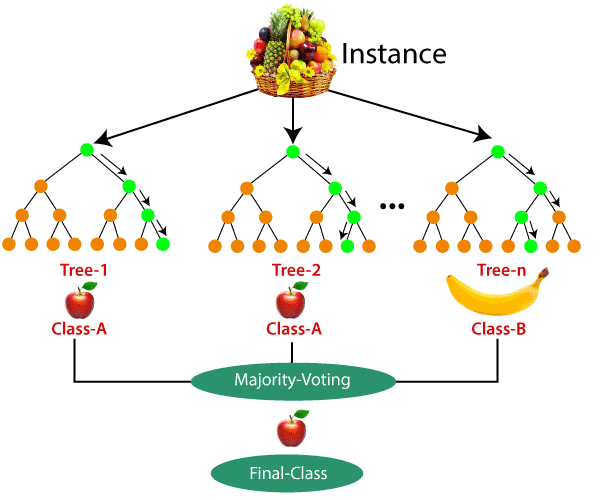
\includegraphics[width=0.8\linewidth]{images/rf_struture.png}
    \caption{Structure of a Random Forest}
    \label{fig:feedforward_structure}
\end{figure}

The algorithm works by creating multiple decision trees, each trained on a random subset of the data and features. For a Random Forest with N trees, the mathematical representation of the final prediction is:

\[
\hat{y} = \frac{1}{N}\sum_{i=1}^{N} f_i(x)
\]
where:
\begin{itemize} 
    \item $\hat{y}$ is the predicted energy consumption value
    \item $f_i(x)$ is the prediction of the i decision tree
    \item $N$ is the total number of trees in the forest
\end{itemize}

Random Forest offers several advantages for energy consumption prediction:

\begin{enumerate}
    \item Feature Importance: It provides insights into which features (e.g., time of day, weather conditions, historical consumption patterns) most significantly impact energy consumption.
    \item Robustness to Outliers: The ensemble nature of Random Forest makes it less sensitive to outliers in the training data.
    \item Handling Non-linearity: It can capture complex non-linear relationships between features and energy consumption without requiring feature transformation.
    \item Reduced Overfitting: By aggregating predictions from multiple trees, Random Forest reduces the risk of overfitting compared to individual decision trees.
\end{enumerate}

The hyperparameters tuned for our Random Forest model include:

\begin{itemize}
    \item Number of trees (n\_estimators)
    \item Maximum depth of trees (max\_depth)
    \item Minimum samples required to split a node (min\_samples\_split)
    \item Minimum samples required at a leaf node (min\_samples\_leaf)
\end{itemize}

\subsection{Feedforward Neural Networks (FNN)}

A Feedforward Neural Network (FNN) is designed to approximate complex functions by mapping input data to output values through a series of hidden layers. For our energy consumption prediction task, the FNN processes information in one direction from the input layer, through the hidden layers, to the output layer without forming cycles or loops.

\begin{figure}[h!]
    \centering
    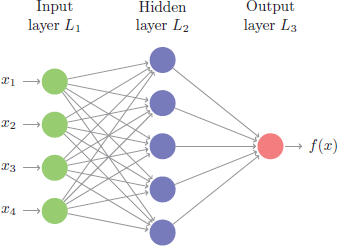
\includegraphics[width=0.8\linewidth]{images/fnn-struture.png}
    \caption{Structure of Feedforward Neural Networks (FNN)}
    \label{fig:feedforward_structure}
\end{figure}

Each neuron in an FNN is a computational unit that applies a weighted sum of its inputs, adds a bias, and passes the result through an activation function. Mathematically, this process can be expressed as:

\[
    y = f(\sum_{i=1}^{N} w_ix_i + b)
\]

where:

\begin{itemize}
    \item $y$ is the neuron's output
    \item $x_i$ are the inputs (features related to energy consumption)
    \item $w_i$ are the weights associated with the inputs
    \item $b$ is the bias term
    \item $f$ is the activation function (e.g., ReLU, Tanh, or Linear)
\end{itemize}

Our FNN architecture consists of three main types of layers:

\begin{enumerate}
    \item Input Layer: This layer receives the input data representing features like historical consumption, weather variables, and other relevant factors.
    \item Hidden Layers: These layers perform the bulk of the computation in the network. Each hidden layer applies a transformation to the data using weights, biases, and activation functions.
    \item Output Layer: This layer produces the network's prediction, which is a single value representing the forecasted energy consumption. For our regression task, the output layer uses a linear activation function.
\end{enumerate}

The training process of our FNN involves:

\begin{itemize}
    \item Forward Propagation: The input data passes through the network layer by layer, with each layer performing its computation.
    \item Loss Calculation: The difference between predicted energy consumption and actual values is measured using Mean Squared Error (MSE).
    \item Backpropagation: The gradient of the loss function with respect to each weight and bias is computed and propagated backward through the network.
    \item Optimization: Adam algorithm updates the weights and biases to minimize the loss, improving the network's predictions.
\end{itemize}

FNNs are well-suited for energy prediction tasks where the relationship between inputs and outputs may be complex and non-linear, but they require careful tuning to avoid overfitting.

\subsection{Long Short-Term Memory (LSTM)}
LSTMs are an extension of recurrent neural networks (RNNs) mainly introduced to handle situations where RNNs fail \cite{g4g_lstm}. These special networks are good at understanding sequences of data - sentences, time series, or music - where the order of inputs matter and predicting the next time step regarding the context of the input. 

The network uses a concept of memory much like the human brain does. For example to fully understand a sentence the brain needs to remember the earlier words to make sense of the next ones.
LSTM networks use a concept of memory through LSTM cells, which are the main difference that distinguish them from RNN networks and are represented in the image \ref{fig:lstm_cell}.

A cell decides what to keep remembering, what to forget, what new information to learn, and what to output. These tasks are handled by three gates: the forget, the input, and the output gates. The forget gate decides what to forget from memory, the input gate decides what new information to add to memory, and the output gate decides what to pass on to the next step. All of these gates in a single cell work together to let the LSTM keep track of relevant information over time, even if the relevant information happened many steps ago.

\begin{figure}[h!]
    \centering
    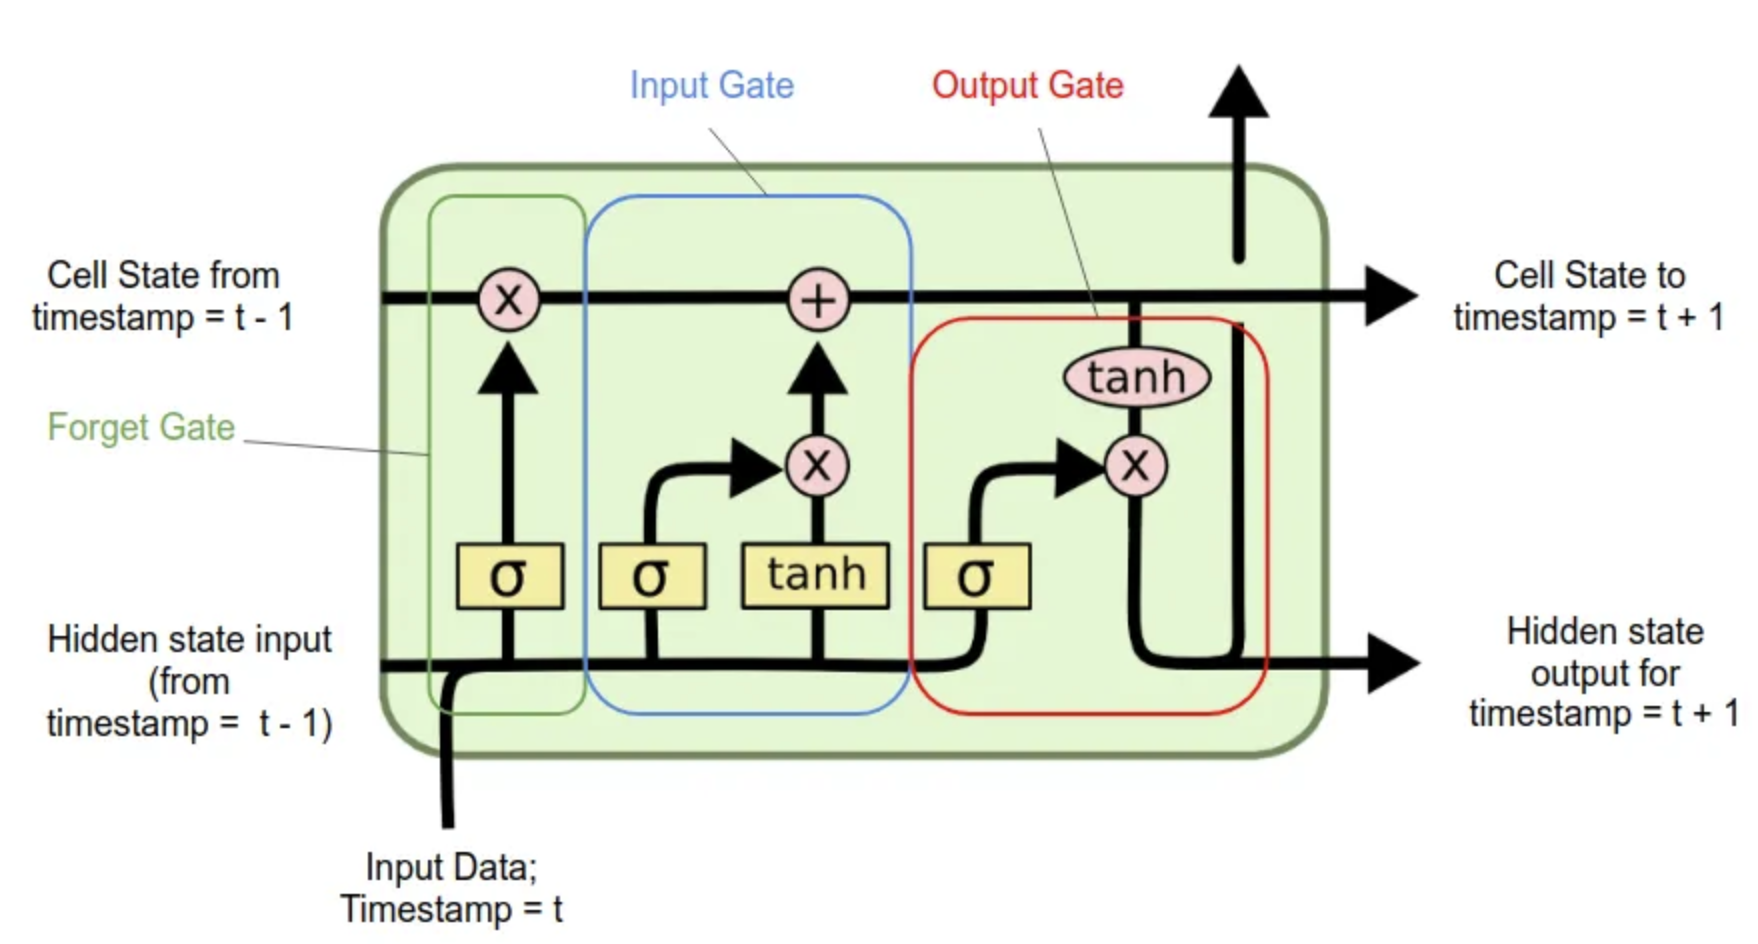
\includegraphics[width=0.8\linewidth]{images/lstm_cell.png}
    \caption{A single LSTM Cell \cite{medium_lstm}.}
    \label{fig:lstm_cell}
\end{figure}

In addition to the gates a single LSTM cell contains the "Cell state" and the "Hidden state". The Cell state encodes a kind of aggregation of data from all previous time steps that have been processed - it can be perceived as the memory of the cell while the Hidden state encodes the data from the most recent time step that has been processed. The Hidden state is not the output (or prediction) but merely an encoding that can be processed to obtain meaningful data.

Each of the gates follows this general equation:
\[f_t = \sigma((W_{hf}\times h_{t-1}) + (W_{xf} \times x) + b_f)\]
The inputs of these equations are \(h_{t-1}\) - a copy of the hidden state from the previous time step, and \(x\) - a copy of the data input at the current time step. The tanh function at the input gate takes another copy of both the hidden state from the previous time step and the data input at the current time step and normalizes it between -1 and 1, instead of 0 and 1 which happens when the sigmoid is applied. 

With each gate's output there is some sort of point-wise or element-wise multiplication which results in a matrix of weights that are between 0 and 1. An example would be that if the forget gate outputs a matrix of values that are all close to 1, it means the forget gate has concluded that based on the current input, the time-series' history is very important, and therefore, when the cell state from the previous time-step is multiplied by the forget gate's output, the cell state continues to retain most of its original value - "remember its past". If the forget gate outputs a matrix of values that are all very close to 0 then the cell state's values are scaled down to small numbers which means the forget gate has told the network to forget most of its past up until the current time-step\cite{medium_lstm}.

\subsection{Data Preprocessing and Hyperparameter Tuning}

To enhance the performance and generalization of the machine learning models, this study employs two critical techniques: data Preprocessing and hyperparameter tuning.

\subsubsection{Data Preprocessing}

For our energy prediction task, proper data preprocessing is essential to improve model performance. The following techniques were applied:

\begin{itemize}
    \item Feature Scaling: All numerical features were standardized or normalized to ensure that no single feature dominates the learning process due to its scale.
    \item Lag Features: Historical energy consumption values at different time lags were incorporated as features to provide context about recent consumption patterns.
    \item Missing Value Handling: Rather than applying imputation methods, we opted for a strict filtering approach. Only buildings with complete time series (from the beginning to the end of the study period) were retained in the dataset. Buildings with gaps or missing values were completely excluded from the analysis, ensuring the integrity and reliability of the data used for training and testing.
    \item Logarithmic Transformation: We applied logarithmic transformation to variables that exhibited heavily skewed distributions. This technique helped normalize the distribution of these variables, reducing the impact of extreme values and improving model performance.
\end{itemize}


\subsubsection{Hyperparameter Tuning}

Hyperparameter tuning involves systematically optimizing the key parameters that govern the training process and architecture of the models. 

Tuning was conducted using techniques like random search to identify the optimal combination of hyperparameters that minimize the validation loss. Cross-validation was employed to ensure robust performance across different subsets of the data.

By integrating comprehensive data preprocessing and hyperparameter tuning into the training workflow, our implemented models are better equipped to handle the challenges of energy consumption prediction, improving accuracy and robustness in the forecasts.


\subsection{Model Evaluation: Regression Metrics}

The evaluation of our energy prediction models was carried out using several regression metrics that provide complementary insights into model performance. These metrics help assess the accuracy, precision, and reliability of our predictions.

\subsubsection{Mean Squared Error (MSE)}

MSE measures the average squared difference between predicted and actual energy consumption values. It gives higher weight to larger errors due to the squaring operation, making it particularly sensitive to outliers.

\[
    MSE = \frac{1}{N}\sum_{i=1}^{N}( y_i - \hat{y_i})^2
\]
where:

\begin{itemize}
    \item $y_i$ is the actual energy consumption
    \item $\hat{y}_i$ is the predicted energy consumption
    \item $n$ is the number of samples
\end{itemize}

\subsubsection{Mean Absolute Error (MAE)}

MAE calculates the average absolute difference between predicted and actual values. It provides an intuitive understanding of prediction error in the same units as the energy consumption being predicted.

\[
    MAE = \frac{1}{N}\sum_{i=1}^{N}|y_i - \hat{y_i}|
\]
where:

\begin{itemize}
    \item $y_i$ is the actual energy consumption
    \item $\hat{y}_i$ is the predicted energy consumption
    \item $n$ is the number of samples
\end{itemize}

\subsubsection{Root Mean Square Error (RMSE)}

RMSE is the square root of the Mean Squared Error, providing a measure of the average magnitude of errors in the same units as the energy consumption being predicted. This makes it particularly interpretable in practical contexts.

\[
    RMSE = \sqrt{\frac{1}{N}\sum_{i=1}^{N}( y_i - \hat{y_i})^2}
\]

\subsubsection{Coefficient of Determination (R²)}

R² indicates the proportion of variance in the dependent variable (energy consumption) that is predictable from the independent variables. It ranges from 0 to 1, with higher values indicating better fit.

\[
    R² =  1 -\frac{\sum_{i=1}^{N}( y_i - \hat{y_i})^2}{\sum_{i=1}^{N}( y_i - \bar{y_i})^2}
\]

This metric provides an intuitive measure of how well the model captures the variations in energy consumption patterns.


\subsubsection{Training Loss}
Training loss quantifies how well the model fits the training data by calculating the difference between predicted and actual values. It is computed using a loss function such as cross-entropy for classification or mean squared error for regression. A lower loss means better model predictions. The goal during training is to minimize loss, but low training loss doesn’t always imply good generalization—overfitting can occur if the model is too closely fit to the training data.

\subsubsection{Visual Evaluation}

In addition to numerical metrics, we created several visualization plots to provide insights into model performance:

\begin{itemize}
    \item Residuals vs Actual Energy Consumption: This plot displays the prediction errors (residuals) on the y-axis against the actual energy consumption values on the x-axis. The ideal pattern shows residuals randomly scattered around the zero line with consistent variance across all energy consumption levels.
    \item Distribution of Prediction Errors: This histogram visualizes the frequency distribution of prediction errors. In an ideal scenario, errors should be centered around zero (indicating unbiased predictions), follow an approximately normal distribution, have minimal spread (narrow distribution) and show few outliers. This plot helps assess whether errors are systematic or random and provides insight into the overall error characteristics. A skewed distribution might suggest that the model consistently over or underestimates energy consumption, while heavy tails indicate frequent large errors.
    \item Predicted vs Actual Energy Consumption: This scatter plot compares predicted energy consumption values (y-axis) against actual observed values (x-axis), with a 45-degree reference line representing perfect predictions. Points should ideally cluster tightly around this line.
    \item Learning Curves:  Plots showing the evolution of MSE, MAE, and R² across training epochs help monitor the training process and identify potential overfitting.
\end{itemize}

By combining these complementary metrics and visualizations, we can thoroughly assess the strengths and weaknesses of each model for energy consumption prediction. This comprehensive evaluation approach guides model selection and further refinement to achieve the most accurate and reliable energy forecasts.
\section{Data Analysis}
\label{sec:Data Analyses}

This study utilizes data from the ASHRAE Great Energy Predictor III Kaggle competition \cite{ashrae-energy-prediction}, a significant data science challenge focused on developing accurate building energy consumption prediction models. The competition provided a comprehensive dataset designed to forecast metered building energy usage across four energy types, with data collected from over 1,000 buildings.

\subsection{Dataset Description}

The original dataset consists of several interconnected files, each serving a specific purpose in the energy prediction task. The primary file, train\.csv, contains historical meter readings with essential columns including building\_id as a foreign key to building metadata, meter type indicators (0 for electricity, 1 for chilled water, 2 for steam, and 3 for hot water), timestamp information for each reading, and the target variable meter\_reading representing actual energy consumption. Complementing this is test\.csv which follows an identical structure but omits the meter\_reading values.

Building characteristics are stored in building\_metadata\.csv, which provides static information about each building. This file includes unique building identifiers, site location codes, primary use categorization (such as education, office, parks or healthcare facilities), square footage information, construction year, and floor count. These attributes provide context for understanding energy consumption patterns across different building types and configurations.

Weather conditions, which significantly influence energy usage, are contained in weather\_train\.csv and weather\_test\.csv for the training and testing periods respectively. These files include site-specific weather measurements captured at regular intervals, featuring air temperature in Celsius, cloud coverage measured in oktas, dew point temperature in Celsius, hourly precipitation depth in millimeters, sea level pressure in millibars, wind direction in degrees, and wind speed in meters per second. This comprehensive weather data enables models to account for environmental factors when predicting energy consumption.


\subsection{Data Pre-Processing}

The data transformation process began with a comprehensive integration of the five CSV files from the original dataset. First, we established relational connections between these files to create a unified analytical base. Initially, building\_metadata\.csv was joined with train\.csv using the building\_id column as the linking key, enriching energy consumption data with building characteristics. Afterward, weather conditions from weather\_train\.csv were incorporated using site\_id and timestamp columns to align environmental factors with corresponding energy readings. 

Following integration, we implemented a filtering criteria to focus exclusively on electricity consumption. By retaining only records where meter = 0, we significantly reduced the dataset size from approximately 20 million to 12 million rows, creating a more focused and manageable dataset while maintaining sufficient data volume for robust analysis. In addition to this filtering, we removed columns demonstrating low predictive power for electricity consumption based on correlation analysis, specifically wind\_direction (correlation: 0.04), wind\_speed (correlation: 0.08), and sea\_level\_pressure (correlation: 0.03), concentrating only on features with demonstrated relevance to electricity consumption prediction.

The dataset contained various patterns of missing values requiring systematic treatment. Weather-related features showed temporal gaps, with air\_temperature missing 4.8\% of values, cloud\_coverage missing 12.3\%, dew\_temperature missing 5.1\%, and precip\_depth\_1\_hr missing 6.7\%. To address these gaps while preserving data characteristics, we implemented a two-step imputation approach: first replacing missing values with the median value for the same site\_id, then filling any remaining missing values with the global median. This methodology preserved site-specific weather patterns while ensuring dataset completeness without introducing artificial anomalies.

Building metadata presented more significant completeness challenges, with year\_built missing in 25.8\% of records and floor\_count absent in 18.4\%. After careful consideration of various approaches, we chose to remove buildings with missing metadata rather than attempt imputation. This decision was based on several key factors: these static, structural features could introduce significant bias if imputed incorrectly; the values are not time-dependent and cannot be reasonably estimated from nearby readings; and even after removal, we retained a sufficiently large dataset (2 million rows) to support robust analysis. This choice prioritized data quality over quantity, reducing the dataset from 12 million to 2 million rows but ensuring higher reliability in the retained data.

To validate our feature selection decisions, we conducted a comprehensive correlation analysis between all potential predictors and electricity consumption. The results confirmed the importance of air\_temperature (0.68 correlation) and square\_feet (0.65 correlation) as primary predictors, with dew\_temperature (0.52), cloud\_coverage (0.23), and precip\_depth\_1\_hr (0.11) also showing meaningful relationships. Based on this analysis, we retained features with correlations above 0.10 and removed others with weaker relationships, as already mentioned before.


\subsection{Data Processing and Data Visualization}

To begin the modeling process, we conducted a thorough pre-processing pipeline that involved cleaning, filtering, engineering new features, and transforming the dataset to ensure quality and consistency.

\subsubsection{Data Cleaning}


We began by converting the timestamp column to datetime format, enabling time-series analysis crucial for energy consumption patterns.

Next, we evaluated the completeness of observations per building. Since the dataset spans hourly readings across an entire year (i.e., 365 days * 24 hours), we expected 8,760 observations per building. However, some buildings had significant gaps, with entire days missing.

\begin{figure}[!h]
    \centering
    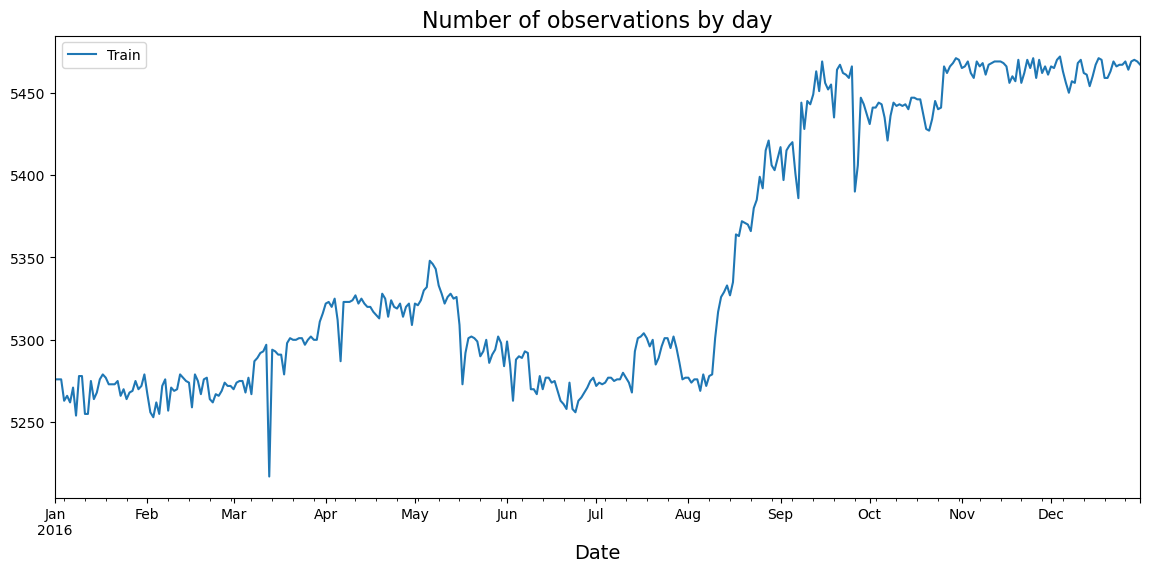
\includegraphics[width=0.75\linewidth]{images/obser_by_day.png}
    \caption{Observations per month with failures}
    \label{fig:obs-by-month-bad}
\end{figure}

To maintain data integrity, we removed buildings with missing target values for entire days, retaining approximately 130 buildings with consistent readings, Fig. \ref{fig:obs-by-month-good}. This resulted in a dataset with around 3,000 observations per day, totaling over one million rows. We then reindexed the dataset to include all combinations of building\_id and timestamp for the year 2016, ensuring temporal continuity.

\begin{figure}[!h]
    \centering
    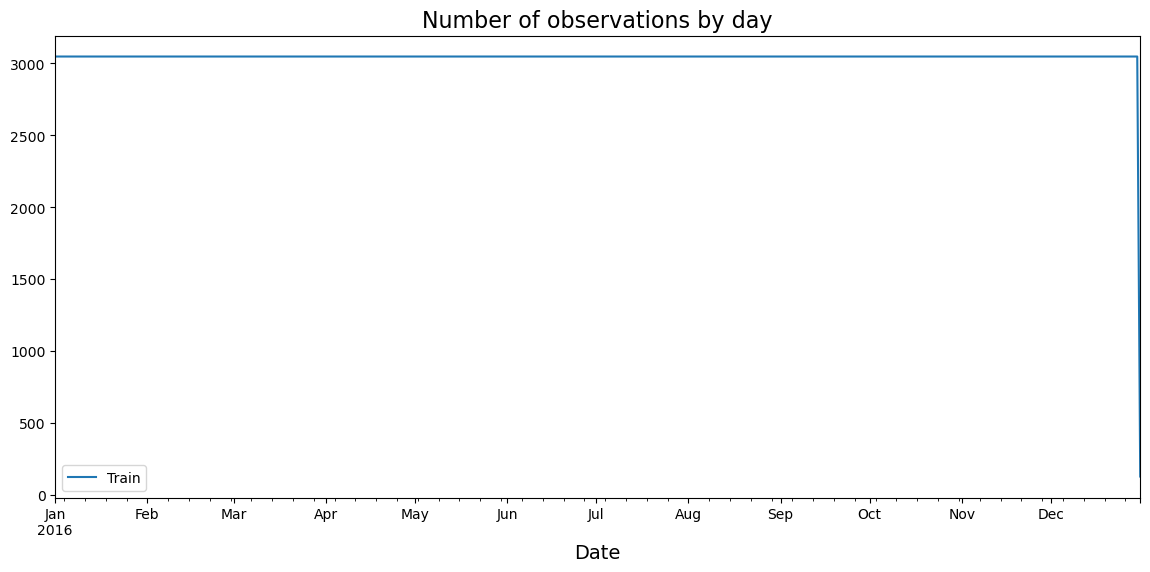
\includegraphics[width=0.75\linewidth]{images/obser-good.png}
    \caption{Observations per month}
    \label{fig:obs-by-month-good}
\end{figure}

We then analyzed the distribution of buildings across the primary\_use categories, Fig. \ref{fig:primary_use_before_delete}. To ensure statistical robustness and avoid sparsity issues, we excluded categories with fewer than 10 unique buildings ('Other', 'Healthcare', 'Manufacturing/industrial'). 

\begin{figure}[!h]
    \centering
    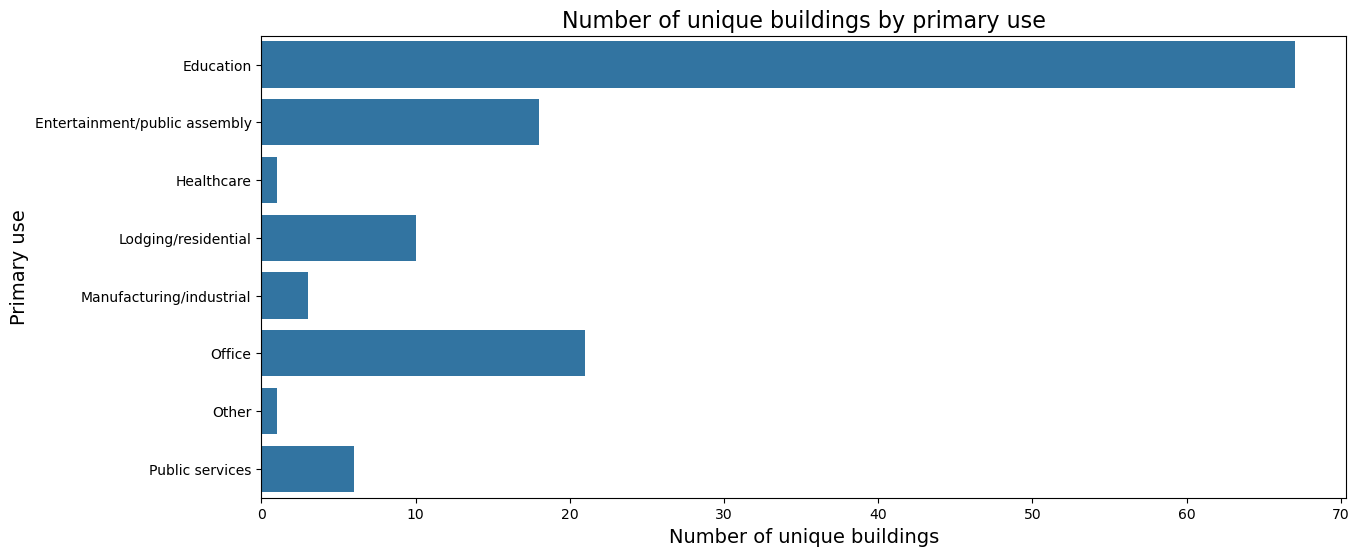
\includegraphics[width=0.75\linewidth]{images/primary_use_after_deleting.png}
    \caption{Number of Unique buildings by Primary Use}
    \label{fig:primary_use_before_delete}
\end{figure}

After this filtering, we performed targeted analysis of the target variable across categories. For instance, we observed that schools and offices had noticeably higher energy consumption, reflecting their more intensive operational schedules, Fig. \ref{fig:energy_consu_by_primary_use}.

\begin{figure}[!h]
    \centering
    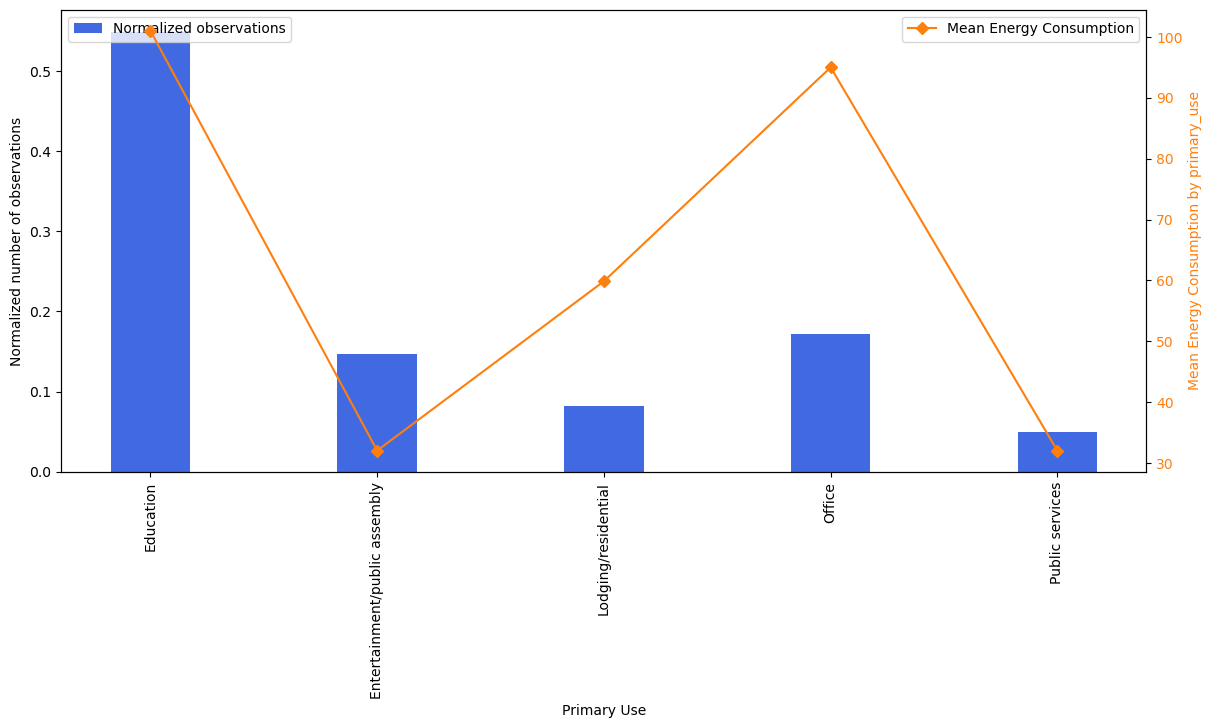
\includegraphics[width=0.75\linewidth]{images/energy_consu_by_primary_use.png}
    \caption{Energy Consumption by primary\_use}
    \label{fig:energy_consu_by_primary_use}
\end{figure}

After, we started by examining the target variable (energy consumption), Fig. \ref{fig:energy_consu_by_site} and air temperature, Fig. \ref{fig:temp_by_site}across different site\_ids. The goal was to assess whether temporal patterns. This preliminary analysis revealed that although some variation existed, the overall structure was sufficiently aligned, allowing for a unified modeling approach across locations.

\begin{figure}[!h]
    \centering
    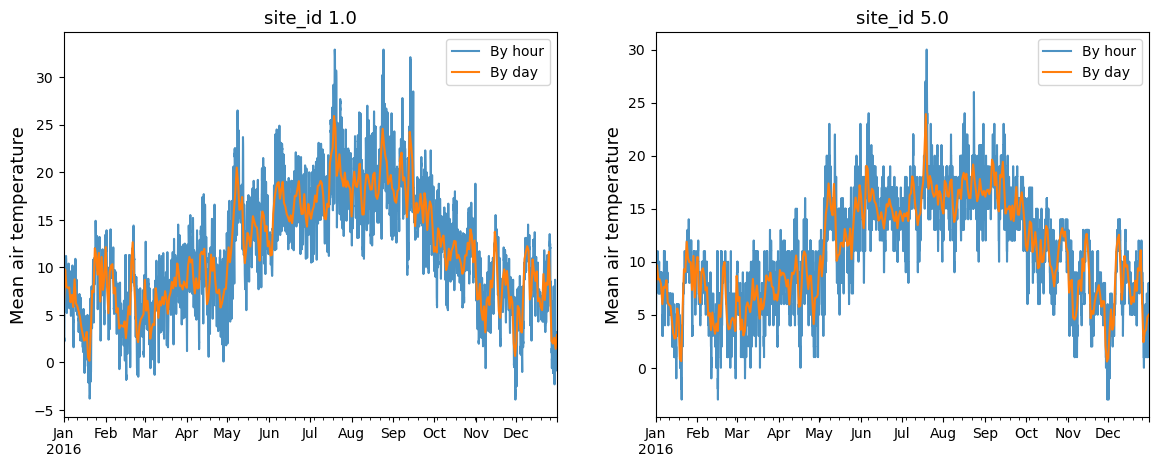
\includegraphics[width=\linewidth]{images/temperature-by-site.png}
    \caption{Air Temperature by Site}
    \label{fig:temp_by_site}
\end{figure}
\begin{figure}[!h]
    \centering
    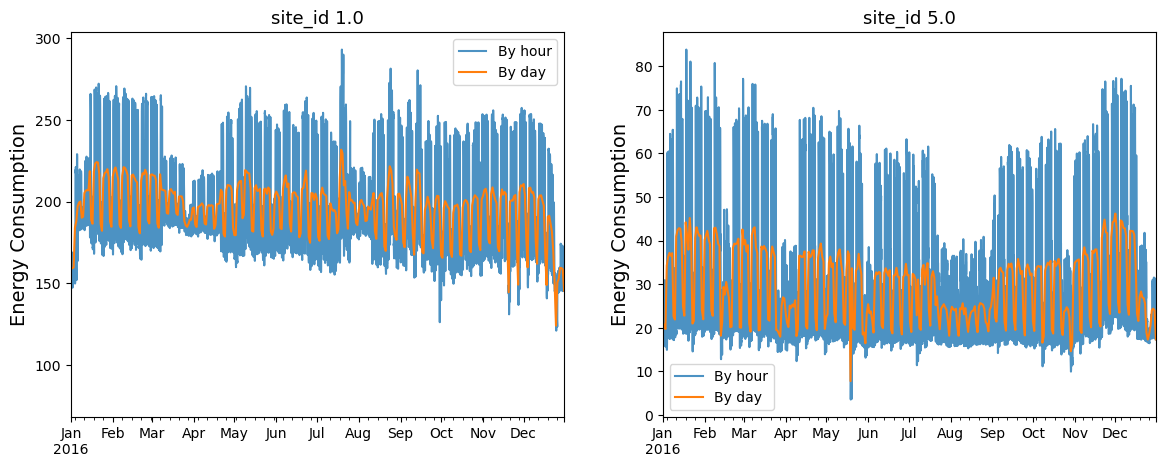
\includegraphics[width=1\linewidth]{images/energy-by-id.png}
    \caption{Energy Consumption by Site}
    \label{fig:energy_consu_by_site}
\end{figure}

\subsubsection{Feature Engineering}
Following the cleaning phase, we moved into feature engineering. We extracted key time-based features from the timestamp column, including hour, day, weekday, and month, to capture daily, weekly, and seasonal consumption cycles. Additionally, we created a new feature, m2\_per\_floor, computed as the ratio between square\_feet and floor\_count, to represent the average area per floor — a potentially useful indicator of spatial density and building efficiency.

Categorical variables required special attention, particularly primary\_use which classifies buildings into functional categories. We applied OneHotEncoder to transform these categorical values into binary representations suitable for machine learning algorithms. This approach preserves the categorical information while avoiding arbitrary ordinal relationships between different building types.

We also engineered a set of lag features for both the target (energy consumption) and air\_temperature, using time lags of 1, 6, 12, 72 (3 days), 120 (5 days), and 168 hours (7 days). These features are essential for capturing temporal dependencies and autoregressive patterns.

\subsubsection{Data Transformation}

\begin{figure}[!h]
    \centering
    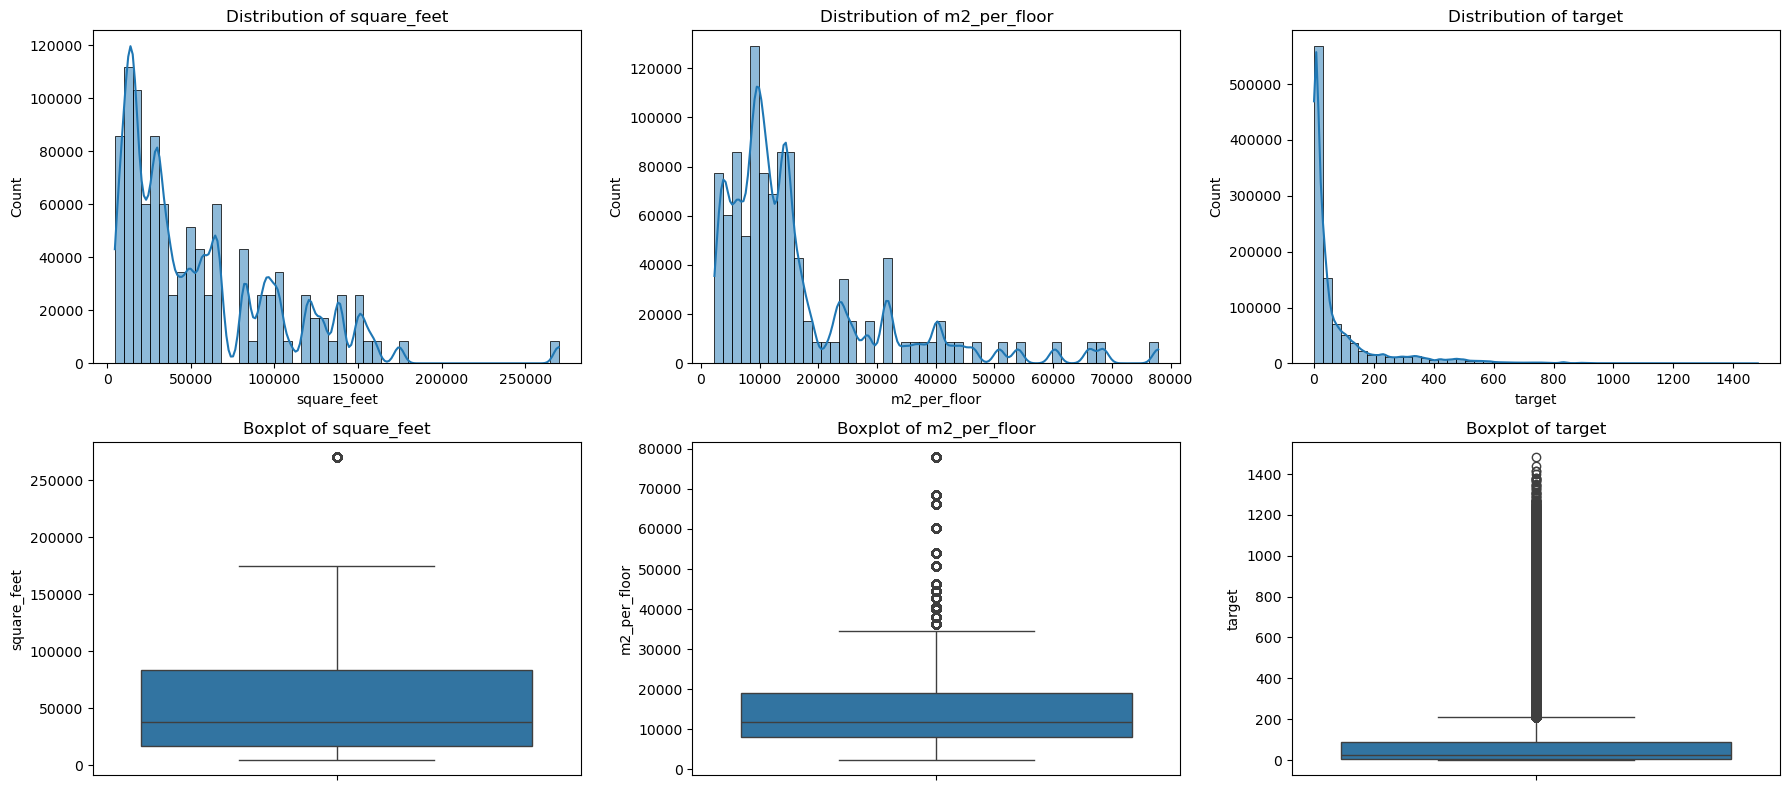
\includegraphics[width=1\linewidth]{images/non-distrib.png}
    \caption{Variables Distributions Before Logarithmic Transformation}
    \label{fig:non-label}
\end{figure}
To address the non-normal distributions evident in Figure \ref{fig:non-label}, we applied logarithmic transformations to several numerical features, including square\_feet, m2\_per\_floor, and the target variable. This transformation effectively compressed the range of large values and expanded the range of small values, resulting in more symmetric distributions that better satisfy the assumptions of many machine learning algorithms, as demonstrated in Figure \ref{fig:Variables Distributions After Logarithmic Transformation}.


\begin{figure}[!h]
\centering
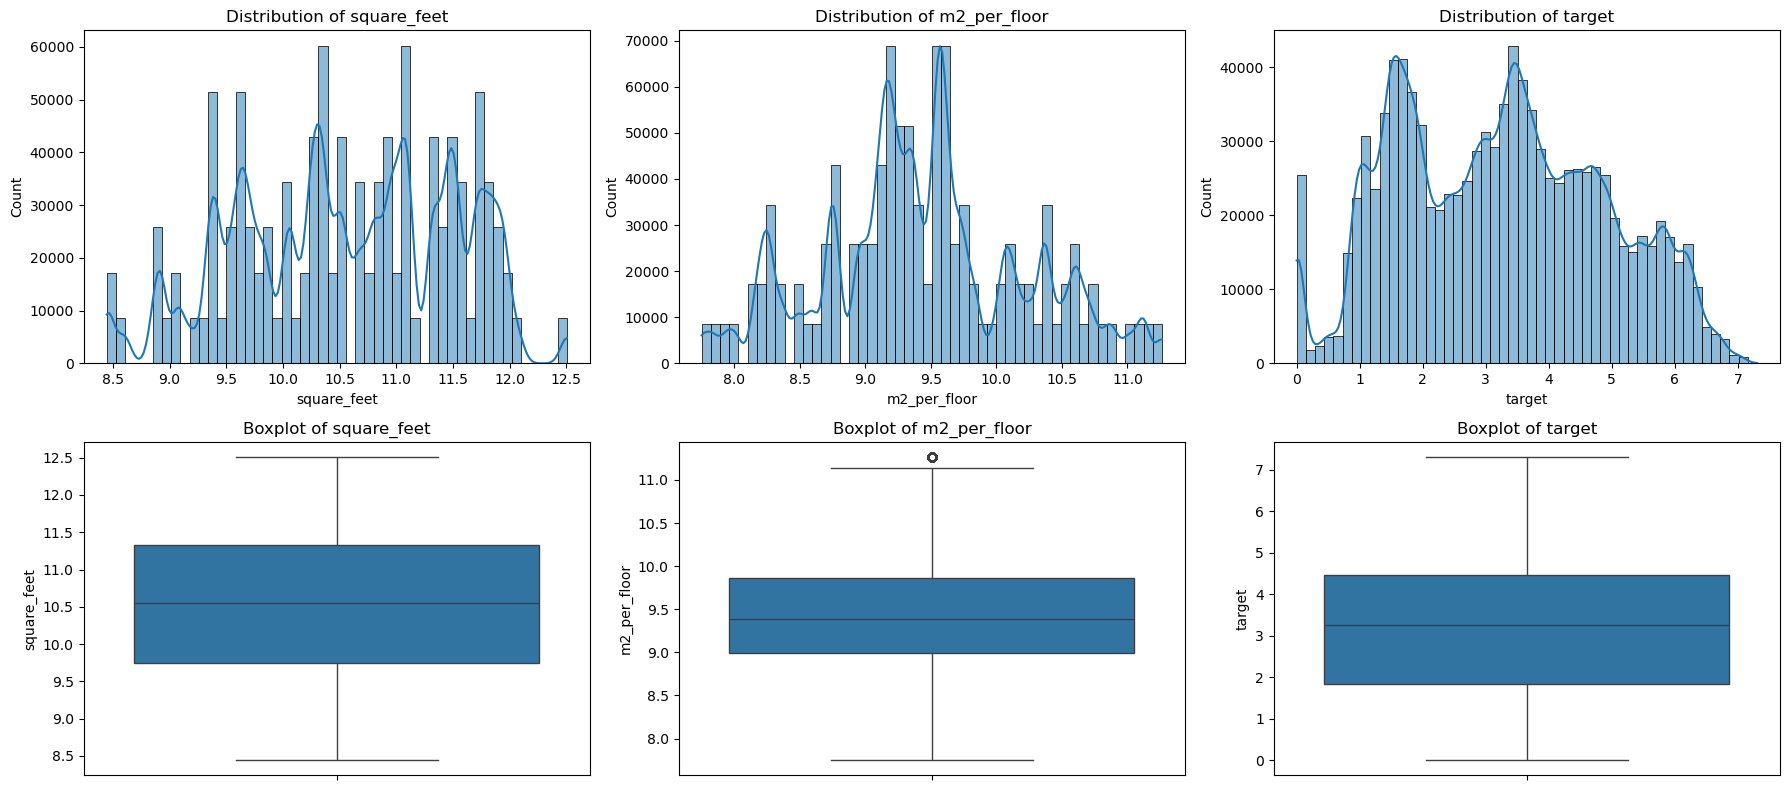
\includegraphics[width=1\linewidth]{images/box_plot-destribution.png}
\caption{Variables Distributions After Logarithmic Transformation}
\label{fig:Variables Distributions After Logarithmic Transformation}
\end{figure}

\begin{figure}[!h]
    \centering
    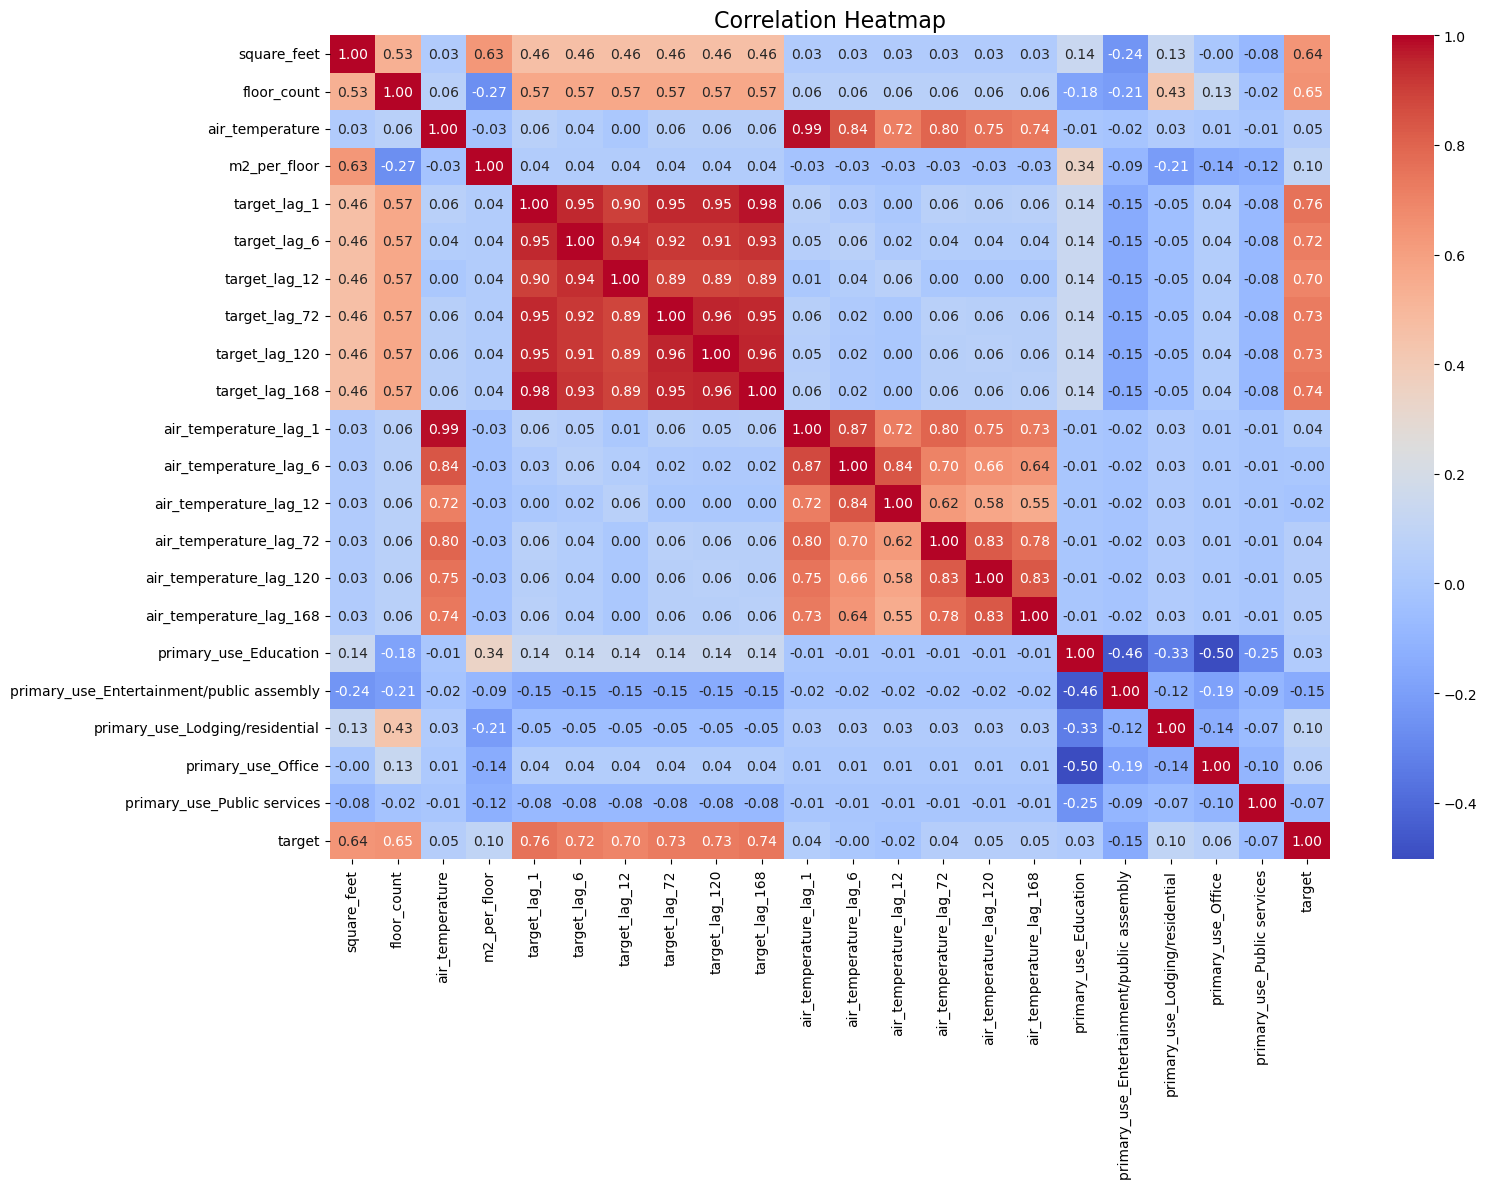
\includegraphics[width=1\linewidth]{images/corr_matrix.png}
    \caption{Correlation Matrix}
    \label{fig:enter-label}
\end{figure}

After feature engineering, we assessed feature importance through correlation analysis and removed variables showing minimal correlation with the target, streamlining the model input space without sacrificing predictive power.


Table \ref{tab:feature_descriptions} presents the complete set of features used in our analysis after preprocessing.

\begin{table}[!h]
\centering
\caption{Feature Descriptions}
\label{tab:feature_descriptions}
\begin{tabular}{|>{\raggedright\arraybackslash}p{2cm}|>{\raggedright\arraybackslash}p{5cm}|}
\hline
\textbf{Feature Name} & \textbf{Feature Description} \\
\hline
\texttt{primary\_use} & The primary functional category of the building (e.g., Education, Office). This feature was one-hot encoded. \\
\texttt{square feet} & Total area of the building in square feet (log-transformed). \\
\texttt{year built} & Year the building was constructed. \\
\texttt{floor count} & Number of floors in the building. \\
\texttt{air temperature} & Hourly air temperature in degrees Celsius. \\
\texttt{m2\_per\_floor} & Average square meters per floor (log-transformed). \\
\texttt{target} & Energy consumption in kilowatt-hours (kWh), measured hourly (log-transformed). \\
\texttt{target\_lag\_1} & Energy consumption 1 hour prior. \\
\texttt{target\_lag\_6} & Energy consumption 6 hours prior. \\
\texttt{target\_lag\_12} & Energy consumption 12 hours prior. \\
\texttt{target\_lag\_72} & Energy consumption 3 days prior. \\
\texttt{target\_lag\_120} & Energy consumption 5 days prior. \\
\texttt{target\_lag\_168} & Energy consumption 7 days prior. \\
\texttt{temp\_lag\_1, ...} & Lagged features for air temperature (e.g., 1h, 6h, etc.). \\
\hline
\end{tabular}
\end{table}


\subsubsection{Data Visualization}

To better understand consumption behavior and uncover temporal patterns in the dataset, we carried out a comprehensive exploratory data visualization phase. This allowed us to contextualize the impact of time, building function, and usage trends on electricity consumption.

We began by computing and visualizing the average energy consumption by hour of the day, day of the month, and day of the week across the entire dataset, Fig. \ref{fig:AvgConsumptionByHour}. The hourly analysis revealed a clear trend: average consumption tends to be significantly higher during standard working hours, approximately between 8:00 and 18:00. This pattern reflects a strong temporal structure tied to building activity cycles, particularly in commercial and institutional buildings.

When grouped by day of the week, the data shows that energy consumption is consistently lower on weekends, supporting the assumption that most buildings are less active during Saturdays and Sundays. This weekly drop is particularly visible in building categories such as Education, Office, and Public Services — which predominantly operate on standard weekday schedules.

\begin{figure}[!h] \centering 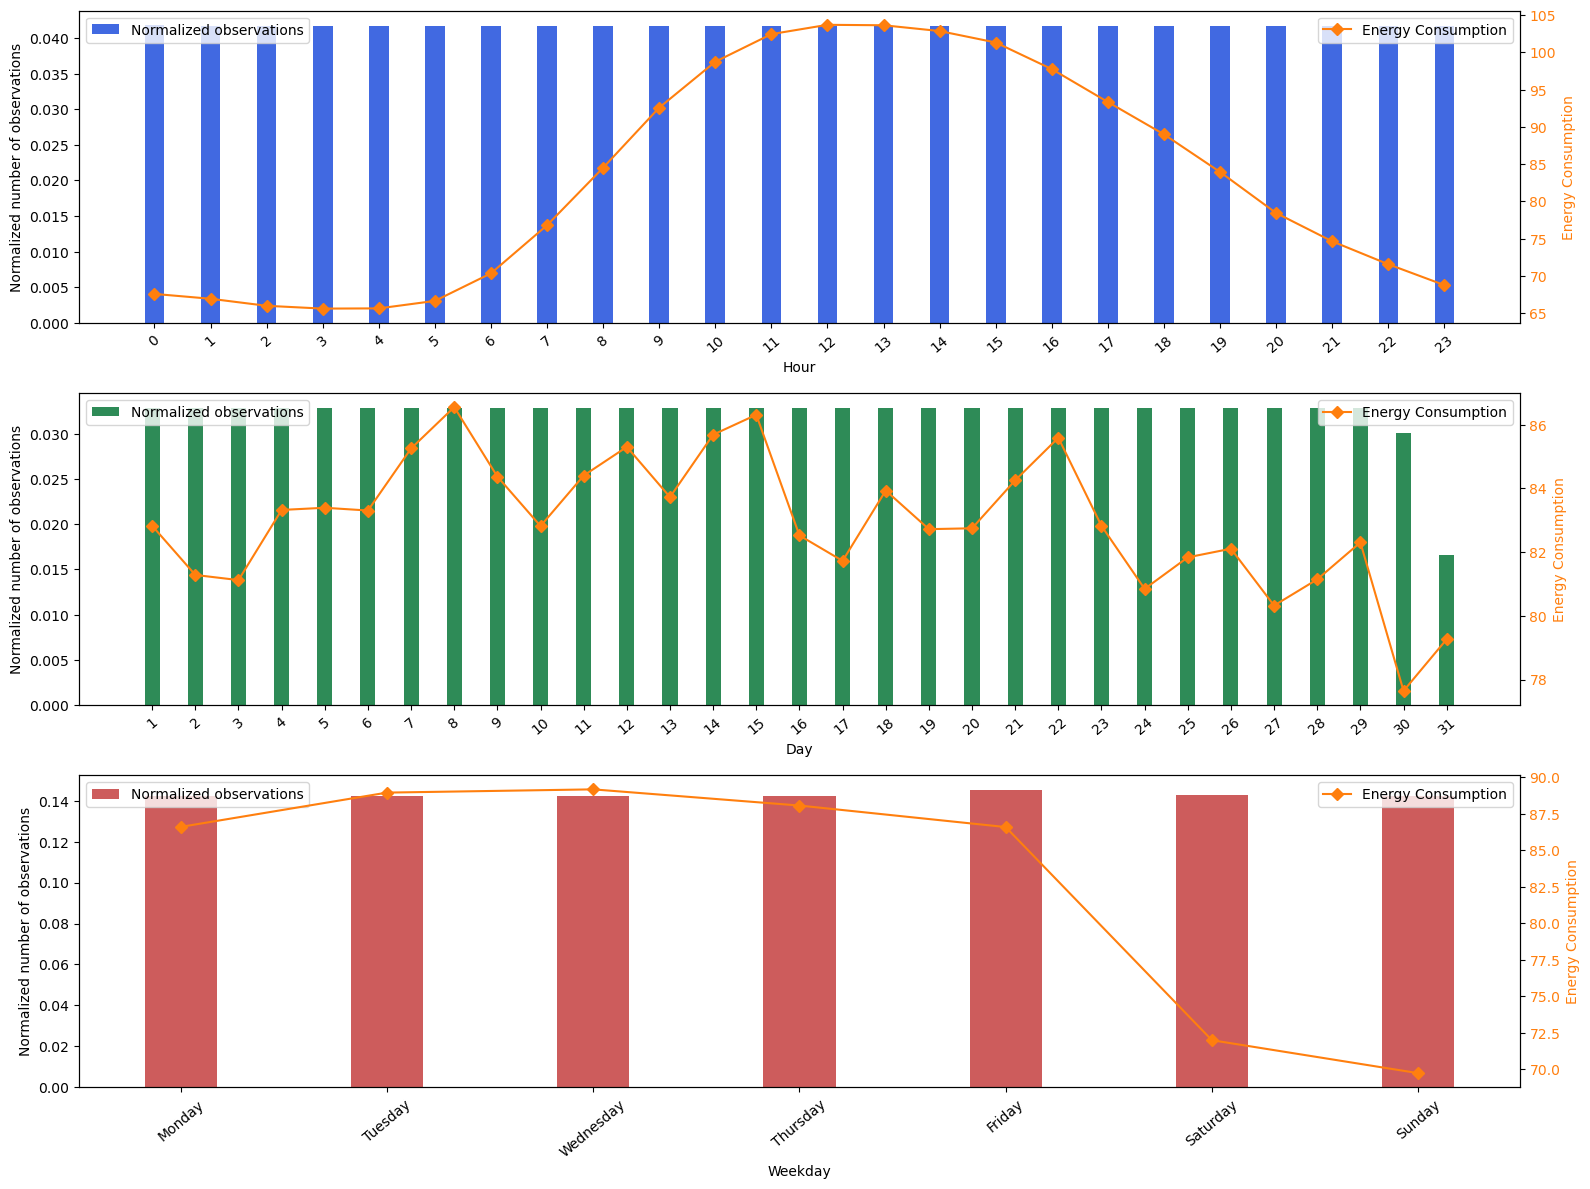
\includegraphics[width=1\linewidth]{images/avg_consumption_by_hour.png} \caption{Average energy consumption by hour of the day (across all buildings)} \label{fig:AvgConsumptionByHour} \end{figure}

\begin{figure}[!h] \centering 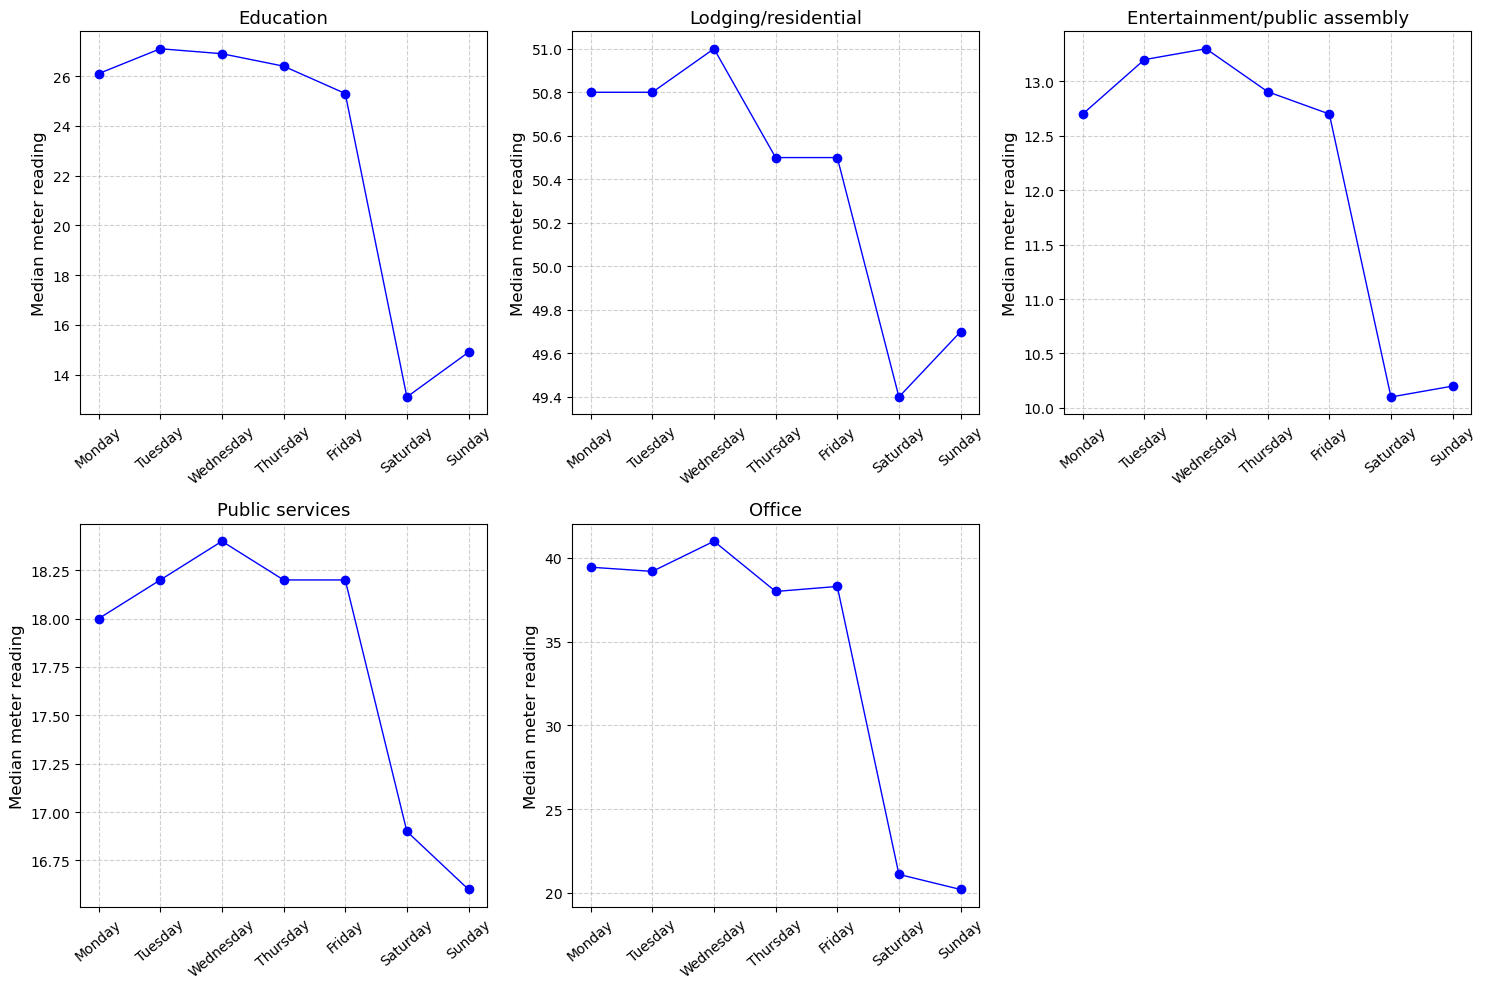
\includegraphics[width=1\linewidth]{images/primary_use_weekly_patterns.png} \caption{Weekly average consumption by primary use category} \label{fig:WeeklyByPrimaryUse} \end{figure}
\begin{figure}[!h] \centering 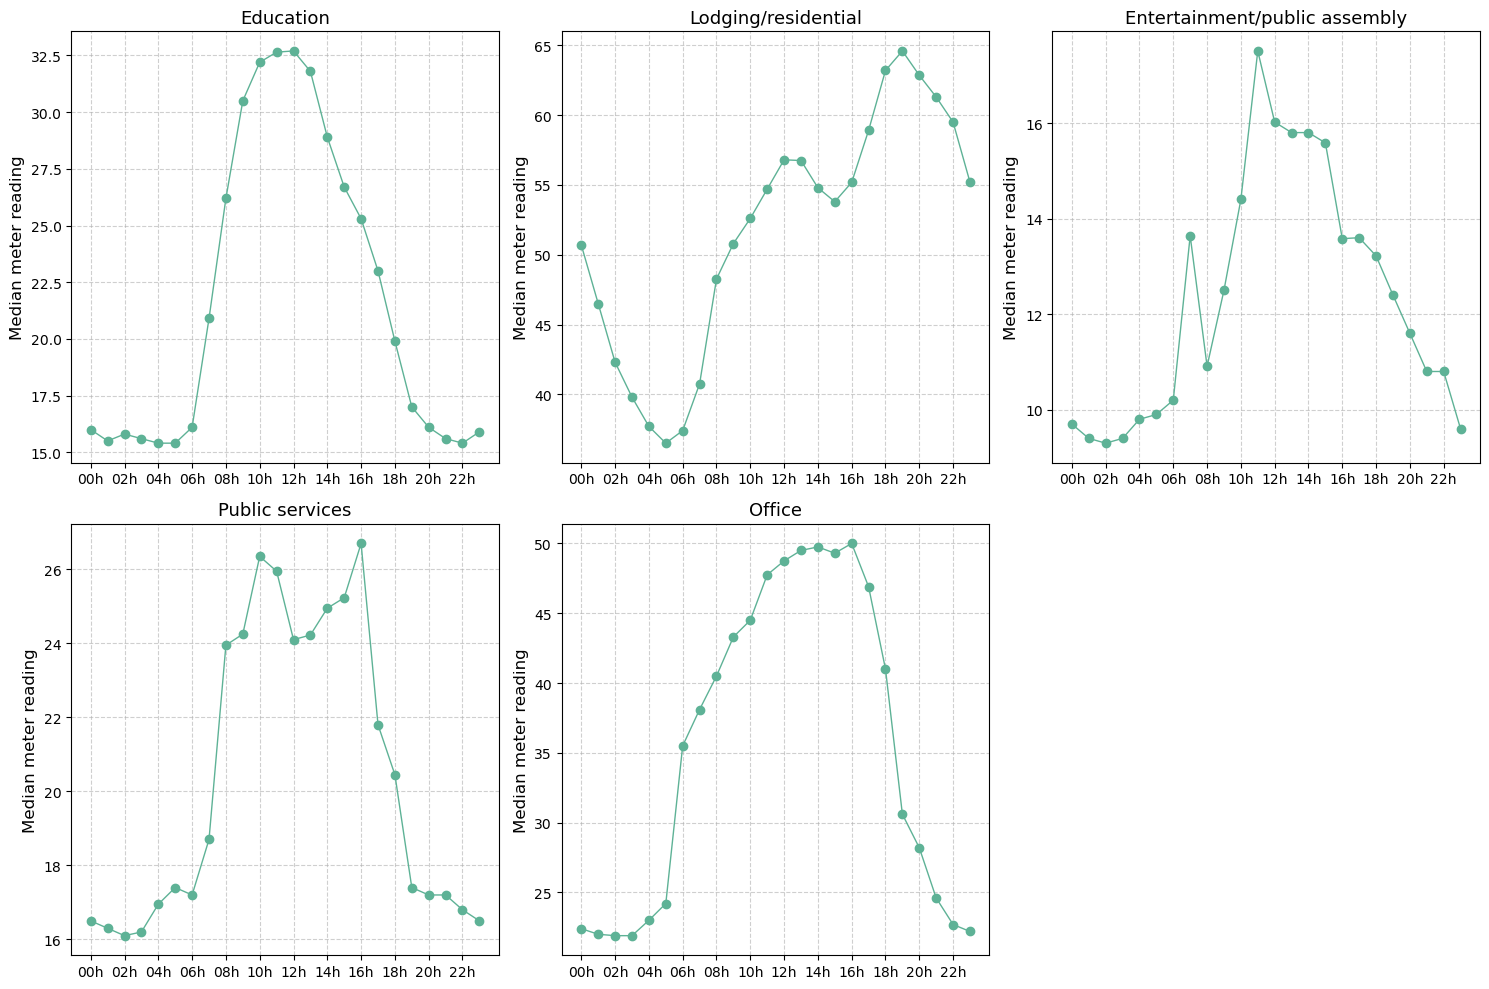
\includegraphics[width=1\linewidth]{images/primary_use_hours_patterns.png} \caption{Hours average consumption by primary use category} \label{fig:HoursByPrimaryUse} \end{figure}

To dig deeper, we disaggregated the data by primary\_use and analyzed the consumption behavior per category throughout the week, Fig. \ref{fig:WeeklyByPrimaryUse} and Fig. \ref{fig:HoursByPrimaryUse}. This comparison made clear that buildings categorized under Education, Public Services, Office, and Entertainment exhibit strong weekday-oriented consumption patterns, with peaks occurring between Monday and Friday from 8 am to 6 pm, and a sharp decline during weekends. These buildings typically operate on fixed schedules and are either closed or underutilized during the weekend.

On the other hand, Residential buildings (e.g., Lodging/Residential) display a different pattern: their energy consumption is more evenly distributed across the week, with subtle peaks during early mornings and evenings — aligning with typical home usage behavior. This contrast highlights how consumption habits differ significantly depending on the building type and its operational hours.

These findings also suggest that the overall weekday consumption bias observed in the aggregate data is likely influenced by the overrepresentation of Education, Office, and Public buildings in the dataset, compared to residential ones.

By identifying these temporal usage patterns and distinguishing between building types, we laid the foundation for time-aware modeling strategies that consider cyclical consumption behaviors — a critical step in improving prediction accuracy and interpretability in energy forecasting tasks.
\section{Results}

In this section, we present the results obtained throughout the development of this work, detailing the different approaches and techniques applied for energy consumption prediction.

Initially, we implemented a Random Forest model as our baseline, applying hyperparameter tuning to optimize performance.

Next, we explored three different feedforward neural network (FNN) architectures:
\begin{enumerate}
\item A simple FNN with minimal layers to establish a neural network baseline.
\item A more complex FNN with additional hidden layers and neurons to capture intricate patterns in the energy consumption data.
\item A specialized FNN that trains different variable groups in distinct ways, allowing the model to process different types of features through specialized network paths.
\end{enumerate}

All FNN models were trained for 50 epochs using the processed dataset that included our engineered features, with particular attention to the lag variables that capture temporal dependencies.

Finally, we implemented a Long Short-Term Memory (LSTM) network, a specialized recurrent neural network architecture designed specifically for sequence prediction problems like our time series energy consumption forecasting. This network was trained for 20 epochs using our processed dataset. The LSTM model leverages its ability to remember patterns over long time intervals, making it particularly well-suited for capturing both short-term fluctuations and long-term trends in energy usage. 

Throughout our experiments, model performance was evaluated using standard regression metrics such as Mean Absolute Error (MAE), Root Mean Squared Error (RMSE), and R² score, allowing for comprehensive comparison across the different methodologies.

\subsection{Random Forest}

The first model developed was a Random Forest, intended to serve as a baseline for the prediction task. To ensure robust evaluation, the dataset was split into training, validation, and test sets using a 60\%/20\%/20\% split, respectively. The split was performed randomly while maintaining a representative distribution across all subsets.

The model's initial performance was evaluated on all three sets: training, validation, and test. Without any hyperparameter tuning, the model already demonstrated excellent performance on the training data, as shown in the table below:

\begin{table}[H]
\centering
\caption{Initial Performance of the Random Forest Model}
\begin{tabular}{||c|c|c|c||}
\hline
\textbf{Metric} & \textbf{Training} & \textbf{Validation} & \textbf{Test} \\
\hline
\textbf{MAE} & 0.0276 & 0.0738 & 0.0734 \\
\hline
\textbf{MSE} & 0.0036 & 0.0253 & 0.0248 \\
\hline
\textbf{RMSE} & 0.0597 & 0.1591 & 0.1576 \\
\hline
\textbf{R²} & 0.9987 & 0.9904 & 0.9906 \\
\hline
\end{tabular}
\label{tab:rf_initial_performance}
\end{table}

The model exhibited near-perfect performance on the training set, with an R² score close to 1. However, performance on the validation and test sets showed a slight decline, indicating that while the model generalized well, there was still room for improvement.

\subsubsection{Hyperparameter Tuning}

To enhance performance and prevent potential overfitting, hyperparameter optimization was performed using \textit{RandomizedSearchCV}. The following parameters were considered during the tuning process:

\begin{itemize}
\item \textit{n\_estimators}: Number of trees in the forest.
\item \textit{max\_depth}: Maximum depth of each tree.
\item \textit{min\_samples\_split}: Minimum number of samples required to split an internal node.
\item \textit{min\_samples\_leaf}: Minimum number of samples required to be at a leaf node.
\item \textit{max\_features}: Number of features to consider when looking for the best split.
\end{itemize}

The best combination of hyperparameters obtained through the search is summarized in the table below:

\begin{table}[H]
\centering
\caption{Best Hyperparameters Found}
\begin{tabular}{|c|c|}
\hline
\textbf{Hyperparameter} & \textbf{Value} \\
\hline
\textit{n\_estimators} & 500 \\
\hline
\textit{min\_samples\_split} & 2 \\
\hline
\textit{min\_samples\_leaf} & 2 \\
\hline
\textit{max\_features} & \textit{log2} \\
\hline
\textit{max\_depth} & \textit{None} \\
\hline
\end{tabular}
\label{tab:rf_best_hyperparameters}
\end{table}

After applying the optimal hyperparameters, the model was re-evaluated. While performance on the training set slightly decreased—indicating reduced overfitting—performance on both validation and test sets improved marginally, suggesting better generalization:

\begin{table}[H]
\centering
\caption{Performance After Hyperparameter Tuning}
\begin{tabular}{||c|c|c|c||}
\hline
\textbf{Metric} & \textbf{Training} & \textbf{Validation} & \textbf{Test} \\
\hline
\textbf{MAE} & 0.0391 & 0.0746 & 0.0744 \\
\hline
\textbf{MSE} & 0.0074 & 0.0238 & 0.0237 \\
\hline
\textbf{RMSE} & 0.0859 & 0.1543 & 0.1541 \\
\hline
\textbf{R²} & 0.9972 & 0.9910 & 0.9910 \\
\hline
\end{tabular}
\label{tab:rf_optimized_performance}
\end{table}

Com os novos hiperparâmetros, o modelo manteve um desempenho elevado e consistente nos três conjuntos. Comparado com a versão inicial, observou-se uma leve redução no desempenho sobre os dados de treino (indicando menor sobreajuste), enquanto os resultados nos conjuntos de validação e teste melhoraram ligeiramente. Isso mostra que o modelo ficou mais robusto e generalizou melhor para dados não vistos.


\begin{figure}[H]
\centering
\begin{minipage}{0.48\textwidth}
  \centering
  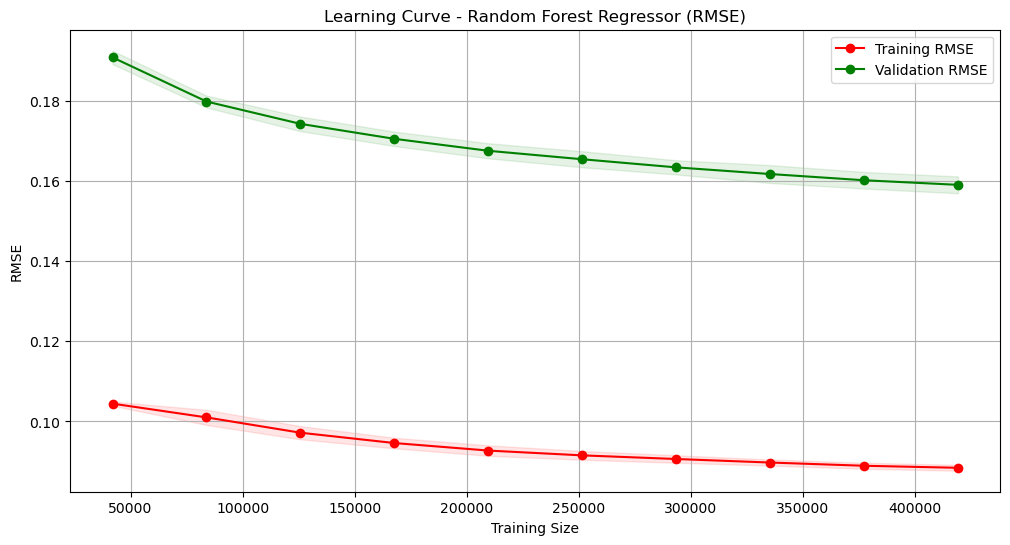
\includegraphics[width=\linewidth]{images/lc-RF-rmse.png}
  \caption{Learning Curve RMSE Random Forest}
  \label{fig:imagem1}
\end{minipage}
\hfill
\begin{minipage}{0.48\textwidth}
  \centering
  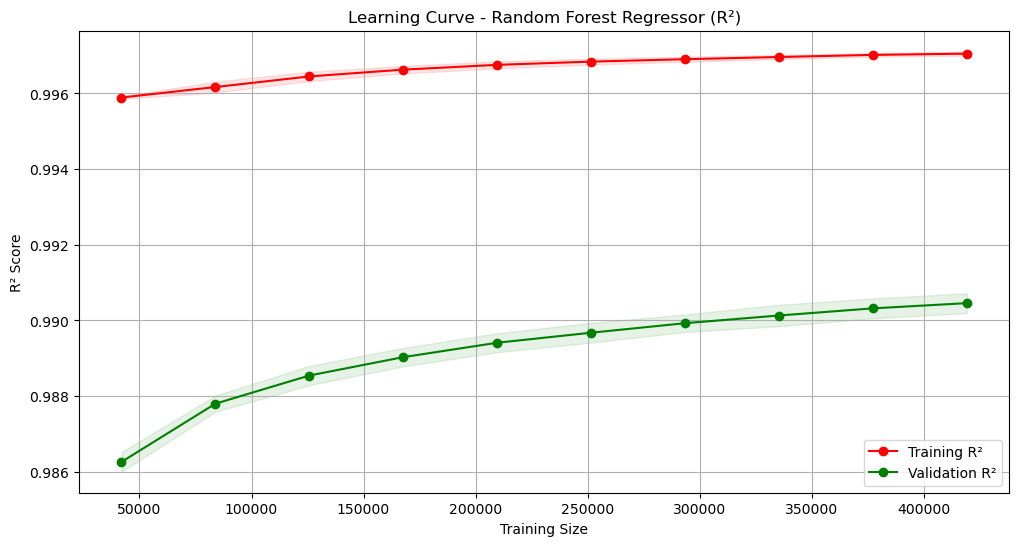
\includegraphics[width=\linewidth]{images/lc-RF-r2.png}
  \caption{Learning Curve $R^2$ Random Forest}
  \label{fig:imagem2}
\end{minipage}
\end{figure}

The learning curves above illustrate the model's behavior during the training process following hyperparameter tuning.

A more detailed analysis of the results shows that the R² score on the training set ranged from 0.994 to 0.998, while on the validation set, it ranged between 0.985 and 0.992. This relatively small difference indicates that the model has strong generalization capabilities, with a low degree of overfitting.

Regarding the RMSE, the values on the training set ranged from 0.12 to 0.07, whereas on the validation set they ranged from 0.19 to 0.15. This discrepancy suggests that the model incurs a slightly higher prediction error on unseen data, although it still maintains robust performance.

Overall, the results demonstrate that the model is well-fitted and generalizes effectively. Nonetheless, there remains some room for improvement in terms of robustness.

\subsection{Feedforward Neural Networks (FNN)}

At this stage, three versions of Feedforward Neural Networks (FNN) were developed, with the objective of comparing different architectures and regularization levels in order to find a balance between performance and generalization. The networks were trained using the Adam optimizer, with the main evaluation metrics being the Mean Absolute Error (MAE), Mean Squared Error (MSE), and the Coefficient of Determination (R²).

The three versions differed in the number of hidden layers, the number of neurons, and regularization techniques such as dropout, and were evaluated on the training, validation, and test sets. The following are the main results obtained for each version.

\subsubsection{FNN 1: Basic Architecture with Dropout Regularization}

The first version of the Feedforward Neural Network (FNN) was designed with a relatively simple architecture, aimed at assessing the performance with moderate regularization using dropout layers. This architecture consists of three dense layers, with 128, 64, and 32 neurons, respectively, and the use of batch normalization to stabilize the training process.

The architecture of the first Feedforward Neural Network (FNN 1) is summarized in the following table:

\begin{table}[h!]
\centering
\caption{Architecture of FNN 1}
\begin{tabular}{|l|c|c|}
\hline
\textbf{Layer\_Type} & \textbf{Output\_Shape} & \textbf{Act\_Function} \\ \hline
Input Layer & (None, input\_dim) & - \\ \hline
Dense Layer (128 neurons) & (None, 128) & ReLU \\ \hline
Batch Normalization & (None, 128) & - \\ \hline
Dropout & (None, 128) & - \\ \hline
Dense Layer (64 neurons) & (None, 64) & ReLU \\ \hline
Batch Normalization & (None, 64) & - \\ \hline
Dropout & (None, 64) & - \\ \hline
Dense Layer (32 neurons) & (None, 32) & ReLU \\ \hline
Dense Output Layer (1 neuron) & (None, 1) & - \\ \hline
\end{tabular}
\label{tab:fnn1_architecture}
\end{table}

The optimizer used is Adam, with a learning rate of 0.001, and the loss function is mean squared error (MSE), appropriate for regression tasks. The metrics monitored during training were MAE, MSE, and R².

\begin{figure}[!h]
    \centering
    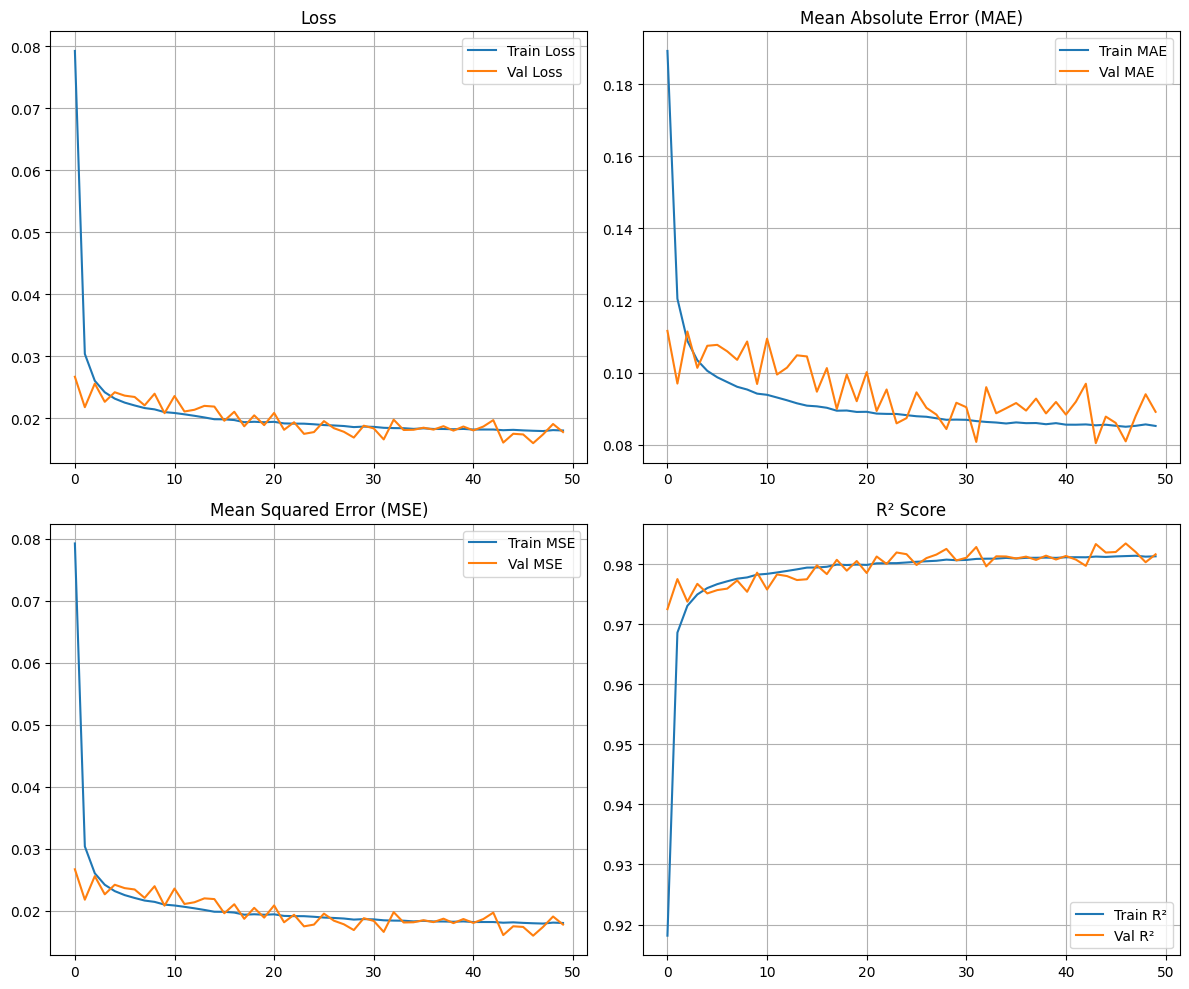
\includegraphics[width=1\linewidth]{images/FNN0-lc.png}
    \caption{FNN 1 learning curves}
    \label{fig:enter-label}
\end{figure}


The learning curves for the first FNN model provide valuable insights into its training behavior and overall performance. The loss curve, shown in the top-left plot, reveals a steep decline in both training and validation loss during the initial epochs. This pattern indicates that the model converged efficiently, learning the underlying patterns in the data without overfitting. The close alignment between training and validation losses further reinforces the model's stability and effectiveness in generalization.

The Mean Absolute Error (MAE) curve, displayed in the top-right, follows a similar trajectory. The error decreases sharply in the early stages and then stabilizes, with training and validation curves closely tracking each other. The absence of significant divergence suggests that the model maintains consistent predictive accuracy across both seen and unseen data, reinforcing its robustness.

Similarly, the Mean Squared Error (MSE), shown in the bottom-left plot, exhibits a rapid decrease followed by stabilization. While the validation MSE presents minor fluctuations, its overall trend remains consistent with the training curve, indicating that the model does not exhibit signs of instability or overfitting.

The R² score curve, presented in the bottom-right, rises quickly during the early epochs and stabilizes above 0.98 after approximately the tenth epoch. The close proximity of the training and validation curves confirms that the model accurately captures the variance in the data and generalizes effectively to new inputs.

In summary, the learning curves collectively indicate that the model is well-tuned and has achieved excellent performance. The consistent behavior across all metrics—loss, MAE, MSE, and R²—demonstrates strong learning capacity and minimal overfitting. 

\begin{table}[H]
\centering
\caption{FNN 1 – Test Set Performance Metrics}
\begin{tabular}{||c|c|c|c|c||}
\hline
\textbf{Metrics} & MAE & MSE & RMSE & R\textsuperscript{2} \\
\hline\hline
\textbf{Values} & 0.1445 & 0.0467 & 0.2161 & 0.9823 \\
\hline
\end{tabular}
\label{tab:fnn1_test_metrics}
\end{table}

The performance on the test set was notably strong, with a Mean Absolute Error (MAE) of 0.1445, Mean Squared Error (MSE) of 0.0467, Root Mean Squared Error (RMSE) of 0.2161, and a Coefficient of Determination (R²) of 0.9823. These results indicate that the model can explain approximately 98.23\% of the variance in the target variable, which is a clear indication of high predictive capability.

The relatively low RMSE suggests that the model's prediction errors are well within acceptable bounds, particularly given the complexity of the data. Combined with the consistent and stable learning curves, these outcomes affirm that the model is both effective and well-generalized. Nonetheless, while FNN 1 achieves robust performance, there remains room for refinement. After this, we explore deeper architectures and alternative regularization strategies to further reduce prediction error and enhance overall robustness.

\begin{figure}[H]
    \centering
    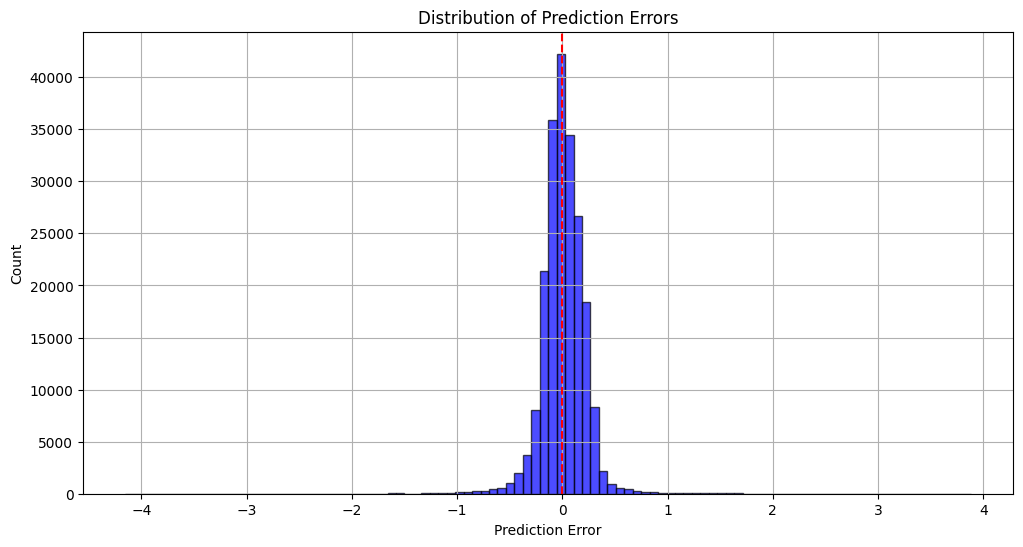
\includegraphics[width=0.8\linewidth]{images/fnn0-de.png}
    \caption{Distribution of Prediction Errors}
    \label{fig:enter-label}
\end{figure}

The histogram of the prediction errors (calculated as actual values minus predicted values) shows a distribution that is centered very close to zero, with the red vertical line likely representing the mean error (0.0090), positioned just slightly above zero. This suggests that the model has minimal bias, as the errors are nearly symmetrically distributed around zero.

The shape of the distribution is approximately normal, which is ideal for a regression model. A normal distribution of errors implies that the model's errors are random, with no obvious patterns, rather than systematic. This indicates that the model is generalizing well and not making consistent mistakes in any specific direction.

The spread of the errors is relatively tight, concentrated between approximately -1 and +1, with very few errors exceeding this range. This suggests that the model's predictions are highly accurate, with most of the predictions being very close to the actual values.

\subsubsection{FNN 2: Deep Architecture with Strong Regularization}

The second Feedforward Neural Network (FNN 2) was designed with a deeper architecture and stronger regularization, aiming to evaluate whether a more complex model could yield better generalization and predictive performance. This version significantly increases the number of layers and neurons, incorporating dropout after each dense layer to mitigate overfitting.

The architecture of FNN 2 is detailed in Table~\ref{tab:fnn2_architecture}.

\begin{table}[h!]
\centering
\caption{Architecture of FNN 2}
\begin{tabular}{|l|c|c|}
\hline
\textbf{Layer\_Type} & \textbf{Output\_Shape} & \textbf{Act\_Function} \\ \hline
Input Layer & (None, input\_dim) & - \\ \hline
Dense Layer (512 neurons) & (None, 512) & ReLU \\ \hline
Batch Normalization & (None, 512) & - \\ \hline
Dropout (0.3) & (None, 512) & - \\ \hline
Dense Layer (256 neurons) & (None, 256) & ReLU \\ \hline
Batch Normalization & (None, 256) & - \\ \hline
Dropout (0.3) & (None, 256) & - \\ \hline
Dense Layer (128 neurons) & (None, 128) & ReLU \\ \hline
Batch Normalization & (None, 128) & - \\ \hline
Dropout (0.3) & (None, 128) & - \\ \hline
Dense Layer (64 neurons) & (None, 64) & ReLU \\ \hline
Batch Normalization & (None, 64) & - \\ \hline
Dropout (0.3) & (None, 64) & - \\ \hline
Dense Layer (32 neurons) & (None, 32) & ReLU \\ \hline
Batch Normalization & (None, 32) & - \\ \hline
Dropout (0.3) & (None, 32) & - \\ \hline
Dense Output Layer (1 neuron) & (None, 1) & - \\ \hline
\end{tabular}
\label{tab:fnn2_architecture}
\end{table}

This model uses the Adam optimizer with a learning rate of 0.001 and is trained to minimize the mean squared error (MSE). The performance metrics monitored throughout training include MAE, MSE, and R².

\begin{figure}[H]
    \centering
    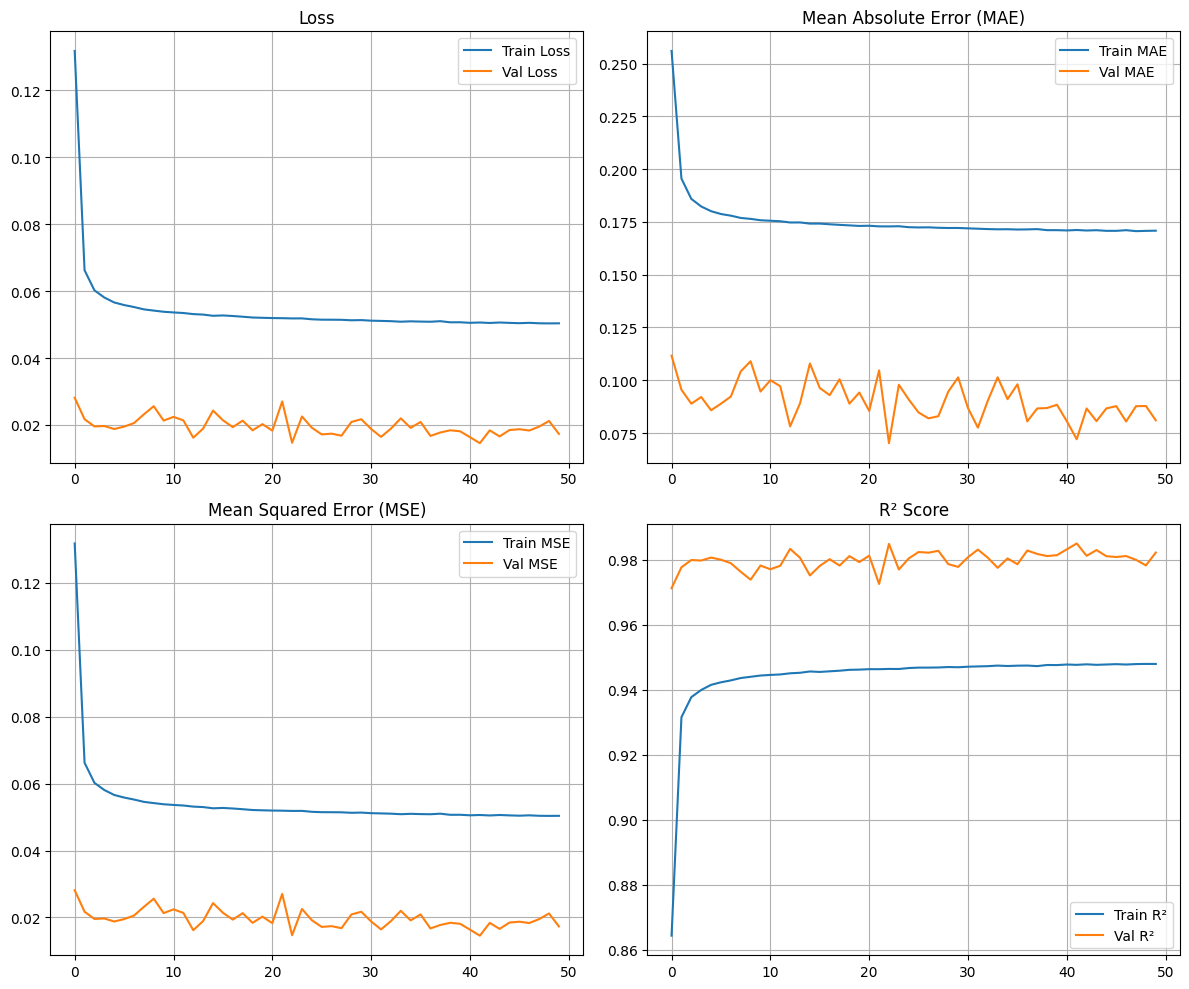
\includegraphics[width=1\linewidth]{images/fnn1-lc.png}
    \caption{FNN 2 learning curves}
    \label{fig:fnn2_learning_curves}
\end{figure}

The learning curves for FNN 2 (Figure~\ref{fig:fnn2_learning_curves}) provide insightful details into the model’s training behavior and its generalization capability. The loss curve (top-left) indicates that the training loss decreases sharply within the first 10 epochs and then stabilizes around 0.05. Notably, the validation loss is consistently lower—hovering around 0.02 throughout training—which is an atypical but encouraging sign that the model generalizes well to unseen data. This consistent gap, where validation outperforms training, suggests an unusual scenario, potentially explained by factors such as data distribution differences or the impact of regularization during training.

The MAE curve (top-right) mirrors the behavior of the loss function. The training MAE decreases and stabilizes at approximately 0.17, whereas the validation MAE remains lower at around 0.09, with minimal fluctuations. The persistent difference indicates that the model is less precise on the training data than on the validation set, a rare occurrence in deep learning. However, the low and stable validation MAE confirms excellent predictive capability on unseen data.

Similarly, the MSE curve (bottom-left) shows that training MSE declines steadily and stabalize near 0.05, while validation MSE holds consistently near 0.02. These results are in line with the loss and MAE plots, reinforcing the conclusion that the model has developed stable predictive power and is not overfitting.

The R² score plot (bottom-right) demonstrates that the training R² begins around 0.86 and gradually increases to stabilize at approximately 0.95. Interestingly, the validation R² starts higher, near 0.975 and remains consistently above the training score throughout the training process. This further supports the notion that the validation set may be easier to predict or exhibits slightly different characteristics than the training data.

In summary, the learning curves of FNN 2 suggest that the model is highly stable, well-regularized, and effective in generalization. All monitored metrics converge after about 10 epochs, implying that additional training is unlikely to yield substantial performance gains. The consistently superior validation performance is atypical and may be attributed to differences in data complexity, sampling strategies, or the effect of dropout and batch normalization disproportionately influencing training dynamics. Nonetheless, the observed behavior indicates that the model is performing reliably across data splits and achieving a high level of accuracy and generalization.

\begin{table}[h!]
\centering
\caption{FNN 2 – Test Set Performance Metrics}
\begin{tabular}{||c|c|c|c|c||}
\hline
\textbf{Metrics} & MAE & MSE & RMSE & R\textsuperscript{2} \\
\hline \hline
\textbf{Values} & 0.1312 & 0.0452 & 0.2125 & 0.9829 \\
\hline
\end{tabular}
\label{tab:fnn2_test_metrics}
\end{table}

The test performance further corroborates the effectiveness of FNN 2. With a Mean Absolute Error of 0.1312, MSE of 0.0452, RMSE of 0.2125, and an R² score of 0.9829, the model clearly demonstrates a high degree of accuracy and a strong ability to explain variance in the target variable. These metrics reflect a slight improvement over FNN 1 and validate the decision to expand the model depth and apply stronger regularization techniques.

\begin{figure}[!h]
    \centering
    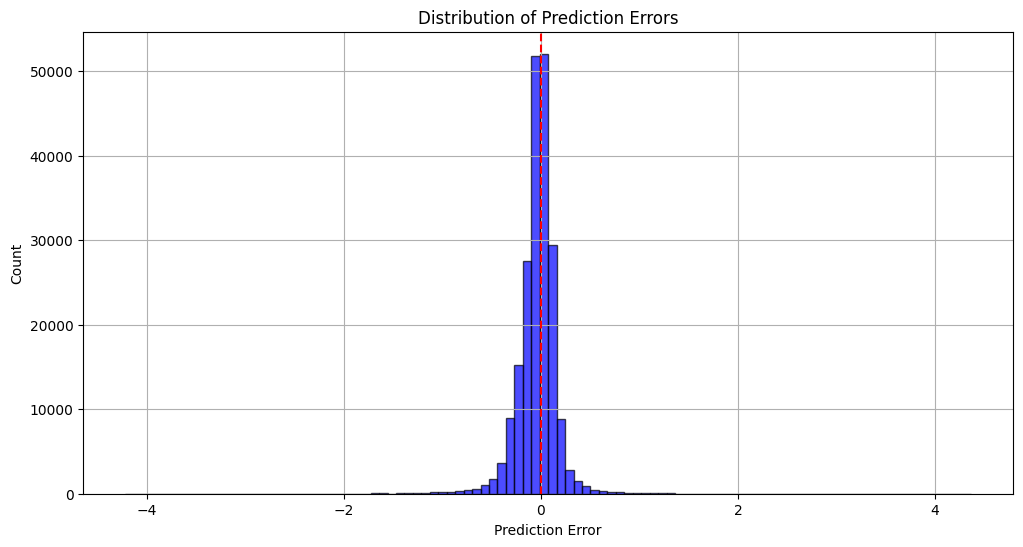
\includegraphics[width=0.8\linewidth]{images/fnn1-de.png}
    \caption{Distribution of Prediction Errors}
    \label{fig:enter-label}
\end{figure}


The errors are centered very near zero, with the red vertical line marking the mean error at approximately \−0.0388. This slight negative shift suggests a minimal and negligible bias in the model's predictions, indicating that, on average, the model slightly overestimates the target values. However, the small magnitude of this bias confirms that the model remains well calibrated overall.

The distribution follows a roughly normal shape, indicating that the model's errors are randomly distributed rather than being systematic. Such a pattern is desirable in regression tasks, as it suggests the absence of structural weaknesses or biases in the model's predictions.

The spread of the errors is narrow, with the majority of predictions falling within a range of approximately \−1 to +1. The standard deviation of the prediction error is 0.2089, reinforcing the model’s consistent accuracy across diverse input conditions. The low variance highlights that most predictions deviate only slightly from the actual values.

\subsubsection{Final Considerations on Tested Architectures}

In addition to the FNN 1 and FNN 2 models detailed earlier, several other experiments were conducted with alternative architectures, including networks with greater depth, different combinations of layers (with and without \textit{Batch Normalization}), and the use of additional regularization techniques like \textit{L2} and \textit{Dropout} in various configurations. However, none of these approaches resulted in significant improvements in the key performance indicators when compared to the two models presented, which proved superior in terms of stability and predictive capability.

Seeking to explore a different approach, a \textit{multi-input model} was also developed, in which the features were logically grouped into sets related to the building, weather variables, temporal lags, and primary use of the building. While this model is simpler in its internal structure, it demonstrated competitive performance on the test set, with \textbf{MAE of 0.1251}, \textbf{MSE of 0.0430}, \textbf{RMSE of 0.2073}, and \textbf{R\textsuperscript{2} of 0.9837}, slightly outperforming the previous models.

Distribution of prediction errors analysis for this model revealed a \textbf{mean error of just 0.0033} and a \textbf{standard deviation of 0.2073}, suggesting not only low bias but also high consistency in predictions. However, due to the grouping of variables into distinct blocks, the learning curves obtained did not provide enough visibility or granularity to allow for a full evaluation of the model’s behavior during training. Despite this visual limitation, the quantitative results demonstrate that the multi-input architecture represents a promising alternative, with potential to be further explored in future work.


\subsection{Long Short-Term Memory (LSTM)}
The last model developed was a simple LSTM network that contained a single LSTM layer which processes the whole temporal sequence. The intuition behind such a simple architecture (of only one layer) is to make comparisons among the previously developed models. An initial training was performed using the default hyperparameters of keras LSTM layer. This model presented great performance metrics when tested.

Right after our first training, we hyper-tuned our model using a grid search approach where the number of units and the recurrent dropout were changed:
\begin{itemize}
    \item num\_units or "hidden size" is analogous to the number of "neurons" in a given layer of a neural network. An LSTM layer contains one or many LSTM cells - the quantity of cells depends on the number of temporal steps. Each of those cells contains a number of units which is defined by the hyperparameter num\_units \cite{ref_num_units}.
    \item The recurrent\_dropout is the fraction of the units to drop for the linear transformation of the recurrent state.
\end{itemize}

The number of units assumed the following values: {32, 64, 128}, and the recurrent dropout assumed the value 0, meaning the recurrent dropout was disabled, and 0.2. After the training phase, the models were tested and the results of the LSTM architecture using the trained hyperparameters is present in the following table.

\begin{table}[H]
\centering
\caption{LSTM model results}
\begin{tabular}{||c|c|c|c|c|c||}
\hline
\textbf{Units} & \textbf{Rec. Dropout} & \textbf{MAE} & \textbf{MSE} & \textbf{RMSE} & \textbf{R²}\\
\hline
32 & 0.0 & 0.111 & 0.041 & 0.203 & 0.984 \\
\hline
32 & 0.2 & 0.105 & 0.039 & 0.198 & 0.985 \\
\hline
64 & 0.0 & 0.104 & 0.037 & 0.191 & 0.986 \\
\hline
64 & 0.2 & 0.098 & 0.034 & 0.184 & 0.987 \\
\hline
128 & 0.0 & 0.096 & 0.032 & 0.179 & 0.988 \\
\hline
128 & 0.2 & 0.093 & 0.032 & 0.180 & 0.988 \\
\hline
\end{tabular}
\label{tab:lstm_performance}
\end{table}

In the table we can see that even though the hyperparameters varied in a quite large range, the test results of our models were very close to each other. Now, taking into consideration the model with the best \(R^2\) let us examine the loss and \(R^2\) performance metric over epochs for both training and validation.

\begin{figure}[H]
    \centering
    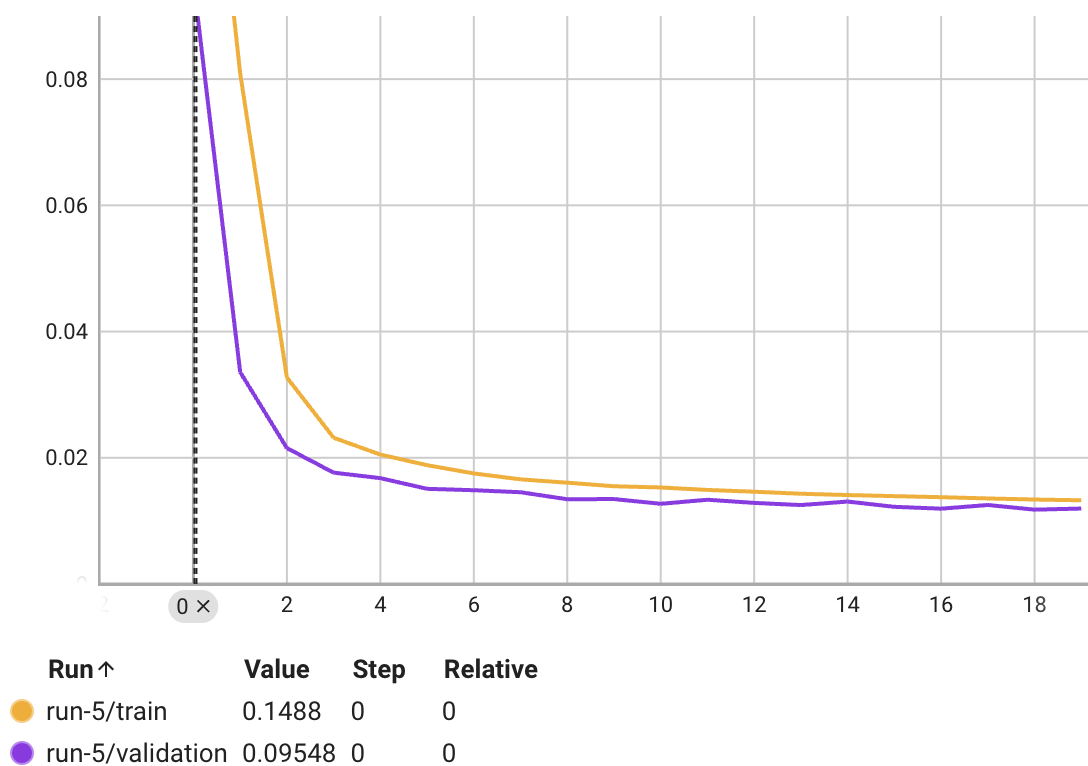
\includegraphics[width=0.75\linewidth]{images/lstm_loss_epoch.png}
    \caption{Loss per epoch}
    \label{fig:lstm_loss_epoch}
\end{figure}
\begin{figure}[H]
    \centering
    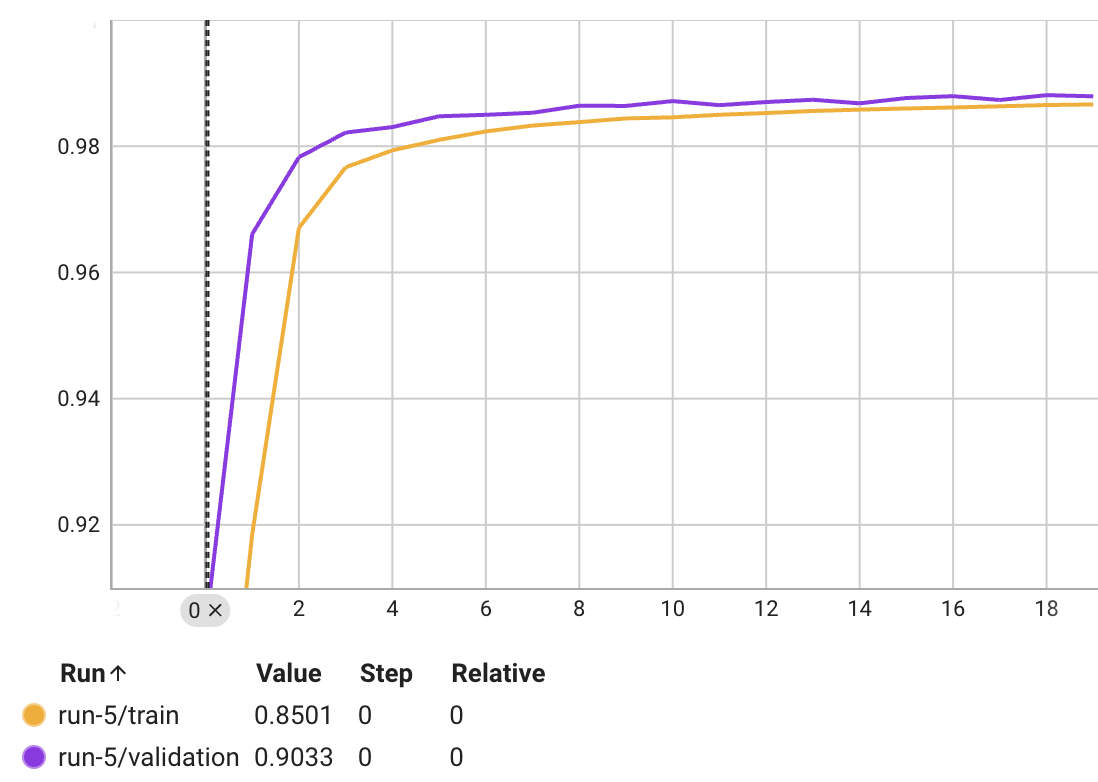
\includegraphics[width=0.75\linewidth]{images/lstm_r2_epoch.png}
    \caption{\(R^2\) per epoch}
    \label{fig:lstm_r2_epoch}
\end{figure}

As seen in the images above, both the loss and \(R^2\) have quickly converged around the fourth epoch. The remaining of the training process seems not to have impact on the performance of our LSTM model. The behaviour of both the validation and training curves suggests optimal learning of the model without signs of overfitting/underfitting.

\section{Comparison with State-of-the-Art Methods}
To evaluate the performance of our models in the context of state-of-the-art solutions, we compared our results to several notable studies. These works employ a diverse range of techniques, from traditional machine learning to advanced deep learning models, allowing us to position our findings within the current research landscape.

\subsection{Short-Term Residential Load Forecasting based
on LSTM Recurrent Neural Network}
In the study "Short-Term Residential Load Forecasting based
on LSTM Recurrent Neural Network"\cite{kong2019short} the authors apply LSTMs to forecast the short-term electricity consumption of individual residential households. 

The authors apply multiple LSTM layers staked on top of each other. These layers are responsible for learning the temporal dependencies between past energy consumption and future predictions. The use of multiple LSTM layers provides the learning of more complex relationships as the depth increases. After the LSTM layers have learned, the output passes through a final feedforward neural network that predicts the energy consumption for the target time step as can be seen in the following image.

\begin{figure}[!h]
    \centering
    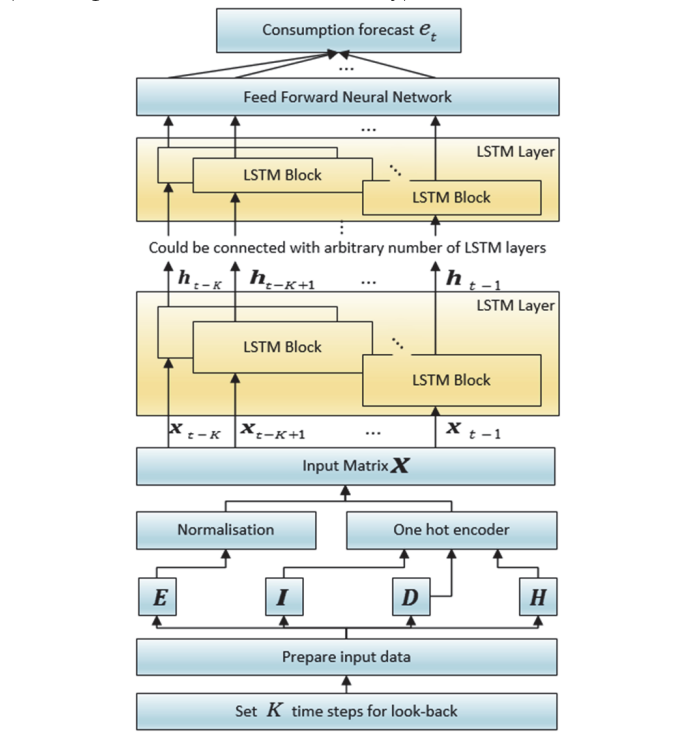
\includegraphics[width=0.75\linewidth]{images/study_lstm.png}
    \caption{Short-term residential load forecasting model architecture\cite{kong2019short}}
    \label{fig:architecture_lstm_study}
\end{figure}

Comparing this architecture with our study's, our architecture is much more simple yet effective for the problem we have at hand. It contains a single LSTM layer, and then a dense layer. Our model has achieved great results and increasing its complexity does not mean we would get better ones. An evidence to this conclusion can be understood from the behaviour of the loss function or \(R^2\) over epochs. We can see the model practically stopped learning in only four epochs which indicates the model is learning very well.

The "Short-Term Residential Load Forecasting(...)" study used the Mean Absolute Percentage Error (MAPE) metric for evaluating the accuracy of the predictions, in contrast to our study which preferred the MAE, MSE, RMSE, and \(R^2\). In conclusion, this comparison highlights that not always a complex model architecture is needed to achieve great results.


\subsection{Comparative Analysis of our results with Existing Studies}

To contextualize the performance of our models, we compare them against notable existing works in the literature. The comparison focuses on key evaluation metrics such as Mean Absolute Error (MAE), Mean Squared Error (MSE), Root Mean Squared Error (RMSE), and the coefficient of determination (R²).

\begin{table}[H]
\centering
\caption{Performance Metrics from Ahmad et al. (2017)~\cite{ahmad2017random}}
\begin{tabular}{llcccc}

 \textbf{Model} & \textbf{RMSE (Val)} & \textbf{R² (Val)} & \textbf{RMSE (Test)} & \textbf{R² (Test)} \\
RF & 0.048 & 0.9968 & 0.0559 & 0.9966 \\
ANN & 0.043 & 0.9975 & 0.0493 & 0.9973 \\
\end{tabular}
\label{tab:ahmad2017_results}
\end{table}

\begin{table}[H]
\centering
\caption{Performance Metrics from Dinh et al. (2023)~\cite{khan2024image}}
\begin{tabular}{llcccc}

\textbf{Dataset} & \textbf{Model} & \textbf{MAE\textsubscript{t}} & \textbf{RMSE\textsubscript{t}} & \textbf{MAE} & \textbf{RMSE} \\

{ DF1} 
& M-LSTM &  0.75  &  1.15  & 1.08 & 1.37 \\
& LSTM   & 1.30 & 1.47 & 1.35 & 1.58 \\
& Bi-LSTM & 1.46 & 1.85 & 1.53 & 1.63 \\
& Linear Reg. & 1.40 & 1.53 & 1.40 & 1.50 \\
{ DF2}  
& M-LSTM &  0.49  &  0.74  & 0.84 & 0.96 \\
& LSTM   & 1.47 & 1.66 & 1.89 & 2.00 \\
& Bi-LSTM & 1.45 & 1.16 & 1.89 & 2.06 \\
& Linear Reg. & 0.60 & 0.75 & 1.21 & 1.52 \\
{ DF3}  
& M-LSTM &  0.66  &  0.85  & 0.69 & 0.87 \\
& LSTM   & 0.79 & 0.95 & 0.67 & 0.94 \\
& Bi-LSTM & 1.61 & 2.15 & 1.23 & 1.92 \\
& Linear Reg. & 0.84 & 1.18 & 0.73 & 0.90 \\

\end{tabular}
\label{tab:dinh2023_results}
\end{table}



\begin{table}[H]
\centering
\caption{Comparison of Test Set Performance Metrics Across our Models}
\begin{tabular}{lcccc}

\textbf{Model} & \textbf{MAE} & \textbf{MSE} & \textbf{RMSE} & \textbf{R²} \\
 Random Forest (Tuned)  & 0.0744 & 0.0237 & 0.1541 & 0.9910 \\
 FNN 1  & 0.1445 & 0.0467 & 0.2161 & 0.9823 \\
 FNN 2  & 0.1312 & 0.0452 & 0.2125 & 0.9829 \\
 FNN with Grouped Features  & 0.1251 & 0.0430 & 0.2073 & 0.9837 \\
 LSTM (Best)  &  0.0930  &  0.0320  &  0.1800  &  0.9880  \\
\end{tabular}
\label{tab:comparison_test_metrics}
\end{table}

Table~\ref{tab:ahmad2017_results} presents the results reported by Ahmad et al. (2017)~\cite{ahmad2017random}, who utilized Random Forest and Artificial Neural Networks (ANN) to predict energy consumption. Their ANN model demonstrated outstanding performance, achieving an RMSE of 0.0493 and an R² of 0.9973 on the test set—surpassing all our models in these two metrics. It is important to note, however, that their experimental setup differs considerably from ours, particularly in terms of input feature types, data resolution, and preprocessing steps. These differences limit the extent to which direct performance comparisons can be made.

In a more recent study, Dinh et al. (2023)~\cite{khan2024image} explored several recurrent neural network variants, including standard LSTM, bidirectional LSTM (Bi-LSTM), and multivariate LSTM (M-LSTM), for time-series forecasting of commercial building energy usage. As shown in Table~\ref{tab:dinh2023_results}, their best-performing models yielded MAEs ranging from 0.49 to 1.53 and RMSEs from 0.74 to 2.06, depending on the dataset. When compared to our best LSTM model (MAE = 0.0930, RMSE = 0.1800), our results demonstrate notably superior accuracy. This improvement may be attributed to targeted preprocessing and feature grouping. Still, such comparisons must be contextualized within the differences in datasets, time horizons, and modeling goals.

Finally, Table~\ref{tab:comparison_test_metrics} summarizes the performance of all our proposed models on the test set. Among them, the tuned Random Forest model achieved the highest R² (0.9910), indicating strong explanatory power. Meanwhile, the LSTM model offered the most balanced performance, combining a low MAE and RMSE with robust generalization. When considered alongside prior studies, our models not only show competitive results but also reinforce the effectiveness of combining classic ensemble methods with modern deep learning techniques in energy consumption prediction tasks.

\section{Future Work}

While the current study demonstrates promising results in predicting energy consumption using various machine learning and deep learning models, several avenues remain for future exploration and improvement.

First, although we focused primarily on unidirectional LSTM architectures, future work could investigate the use of \textbf{Bidirectional LSTM (Bi-LSTM)} and \textbf{Multivariate LSTM (M-LSTM)} models. These architectures have shown potential in related literature for capturing complex temporal dependencies by incorporating both forward and backward sequences, as well as leveraging multiple input features more effectively. Given our positive results with grouped features, a multivariate time-series approach could further improve model accuracy and robustness.

Additionally, our current models were trained on a unified dataset that includes buildings with a variety of \textbf{primary use types}. This generalization can limit performance, especially if usage patterns vary significantly between categories (e.g., schools vs. hospitals vs. offices). A logical extension of our work would involve \textbf{training specialized models per primary use category}, allowing each model to learn domain-specific patterns and seasonal trends. This segmentation could lead to more precise and tailored energy forecasts.

In summary, the foundation laid by this study can be expanded upon through architectural innovations, data stratification, and richer contextual inputs, paving the way for even more accurate and adaptive energy forecasting models.

\input{3-conclusão}
% printing acronyms
\printglossary[type=\acronymtype,title=Acronyms]

% references section
\bibliography{refs}
\bibliographystyle{IEEEtran}



\end{document}